\chapter{Качество переходных процессов}
\label{ch:chap2}

\ExplSyntaxOn
\clist_new:N \l_feq_vector_clist
\NewDocumentCommand{\feqvector}{O{\\}mO{b}}{
  \clist_set:Nn \l_feq_vector_clist {#2} % Set the list
  \begin{#3matrix}
  \clist_use:Nn \l_feq_vector_clist {#1} % show it with separator from #1 (\\)
  \end{#3matrix}
}
\ExplSyntaxOff

Дана система третьего порядка, заданная передаточной функцией:
$$
W(s) = \frac{|\lambda_1\lambda_2\lambda_3|}{(s-\lambda_1)(s-\lambda_2)(s-\lambda_3)}
$$

Тогда найдём динамическую систему, соответствующую передаточной функции:


$$
\begin{aligned}
  y = W(s)u \\
  y = \frac{|\lambda_1\lambda_2\lambda_3|}{(s-\lambda_1)(s-\lambda_2)(s-\lambda_3)} u \\
  (s-\lambda_1)(s-\lambda_2)(s-\lambda_3)y = |\lambda_1\lambda_2\lambda_3| u  \\
  s^3 - (\lambda_1 + \lambda_2 + \lambda_3)s^2 + (\lambda_2\lambda_1 + \lambda_3\lambda_2 + \lambda_3\lambda_1)s - \lambda_1\lambda_2\lambda_3 = |\lambda_1\lambda_2\lambda_3| u  
\end{aligned}
$$

Но для упрощения моделирования будем подавать простой вход $u(t) = 1$ и использовать простой блок передаточной функции в $\textit{simulink}$:
\begin{figure}[ht]
    \centering
    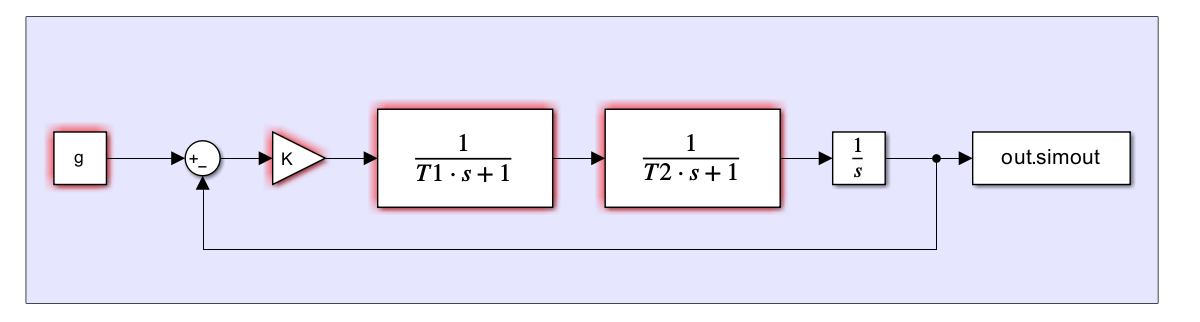
\includegraphics[width=1.0\textwidth]{scheme_system2.png}
  \caption{Схема - задание 2}
\end{figure}


\newpage
\section{1-й эксперимент}
\begin{figure}[ht]
    \centering
    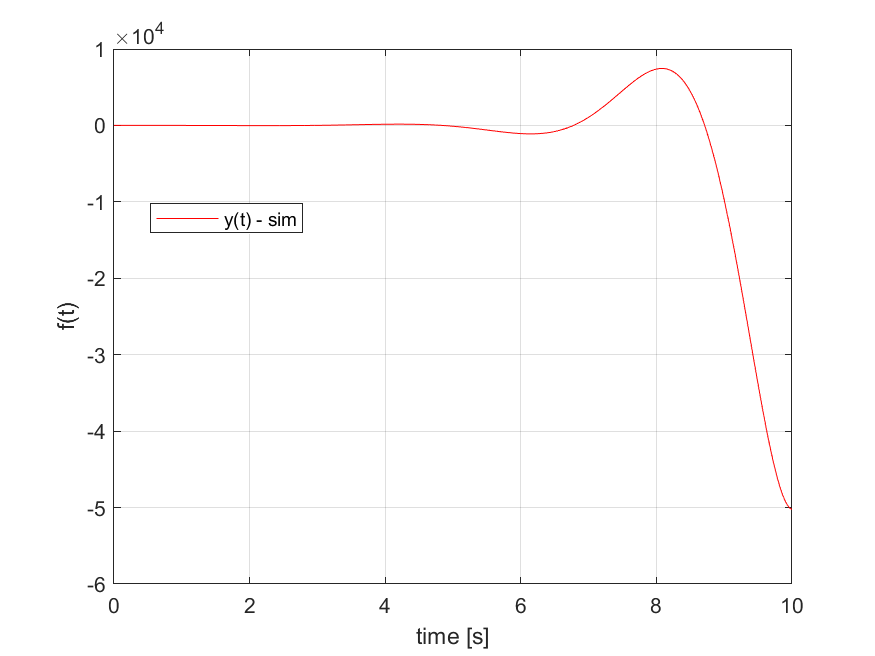
\includegraphics[width=0.8\textwidth]{output_task2_exp1.png}
  \caption{Симуляция - при $\lambda_1 = -1, \lambda_2 = -2,\lambda_3 = -3$}
\end{figure}
Для подсчёта перерегулирования(overshoot) системы воспользуемся классической формулой с ВПД:
$$
\sigma = \frac{y_{max} - y_{final}}{y_{final}}\cdot 100\%
$$
Время переходного процесса будет заканчиваться в нашем случае при попадании в порог $\approx97\%$ от финального значения.
Дальше я не буду дублировать эти формулы, а сразу буду писать результат.
$$
\begin{aligned}
  \sigma_1 \approx 0\% \\
  t_1 \approx 5.1s
\end{aligned}
$$

\newpage
\section{2-й эксперимент}
\begin{figure}[ht]
    \centering
    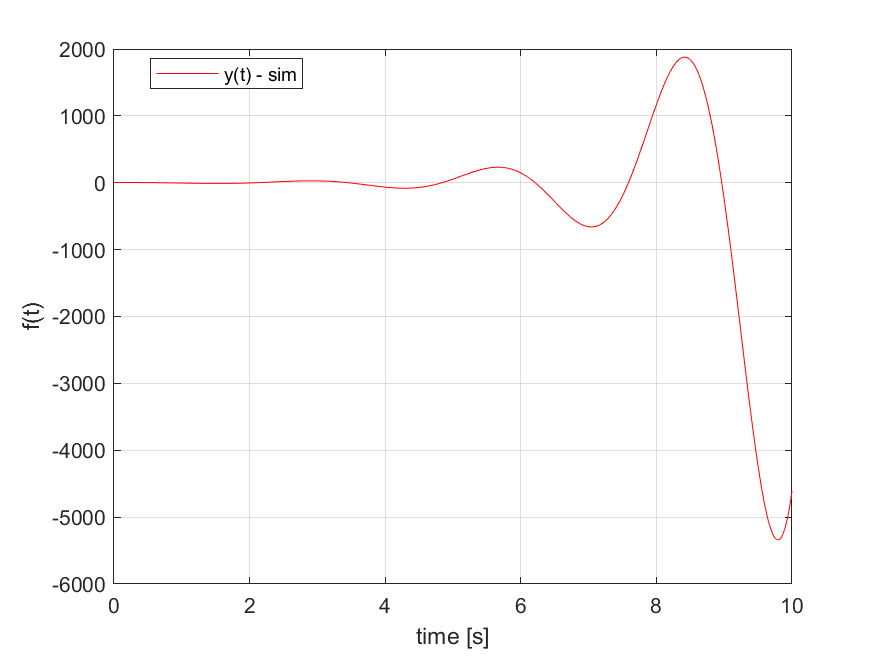
\includegraphics[width=0.8\textwidth]{output_task2_exp2.png}
  \caption{Симуляция - при $\lambda_1 = -1, \lambda_2 = -2,\lambda_3 = -10$}
\end{figure}
Получаем:
$$
\begin{aligned}
  \sigma_2 \approx 0\% \\
  t_2 \approx 4.8s
\end{aligned}
$$

\newpage
\section{3-й эксперимент}
\begin{figure}[ht]
    \centering
    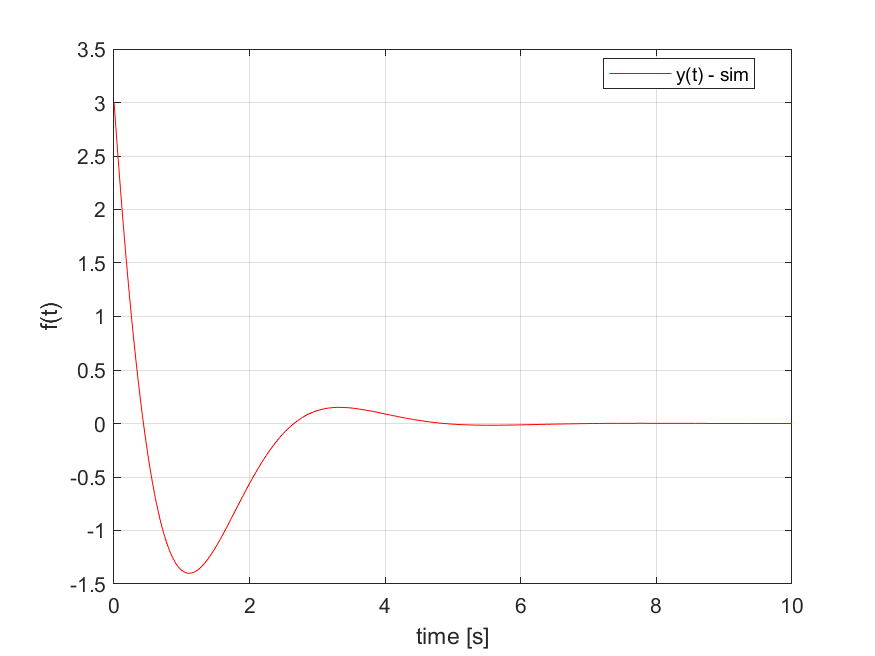
\includegraphics[width=0.8\textwidth]{output_task2_exp3.png}
  \caption{Симуляция - при $\lambda_1 = -10, \lambda_2 = -2,\lambda_3 = -3$}
\end{figure}
Получаем:
$$
\begin{aligned}
  \sigma_3 \approx 0\% \\
  t_3 \approx 2.7s
\end{aligned}
$$

\newpage
\section{4-й эксперимент}
\begin{figure}[ht]
    \centering
    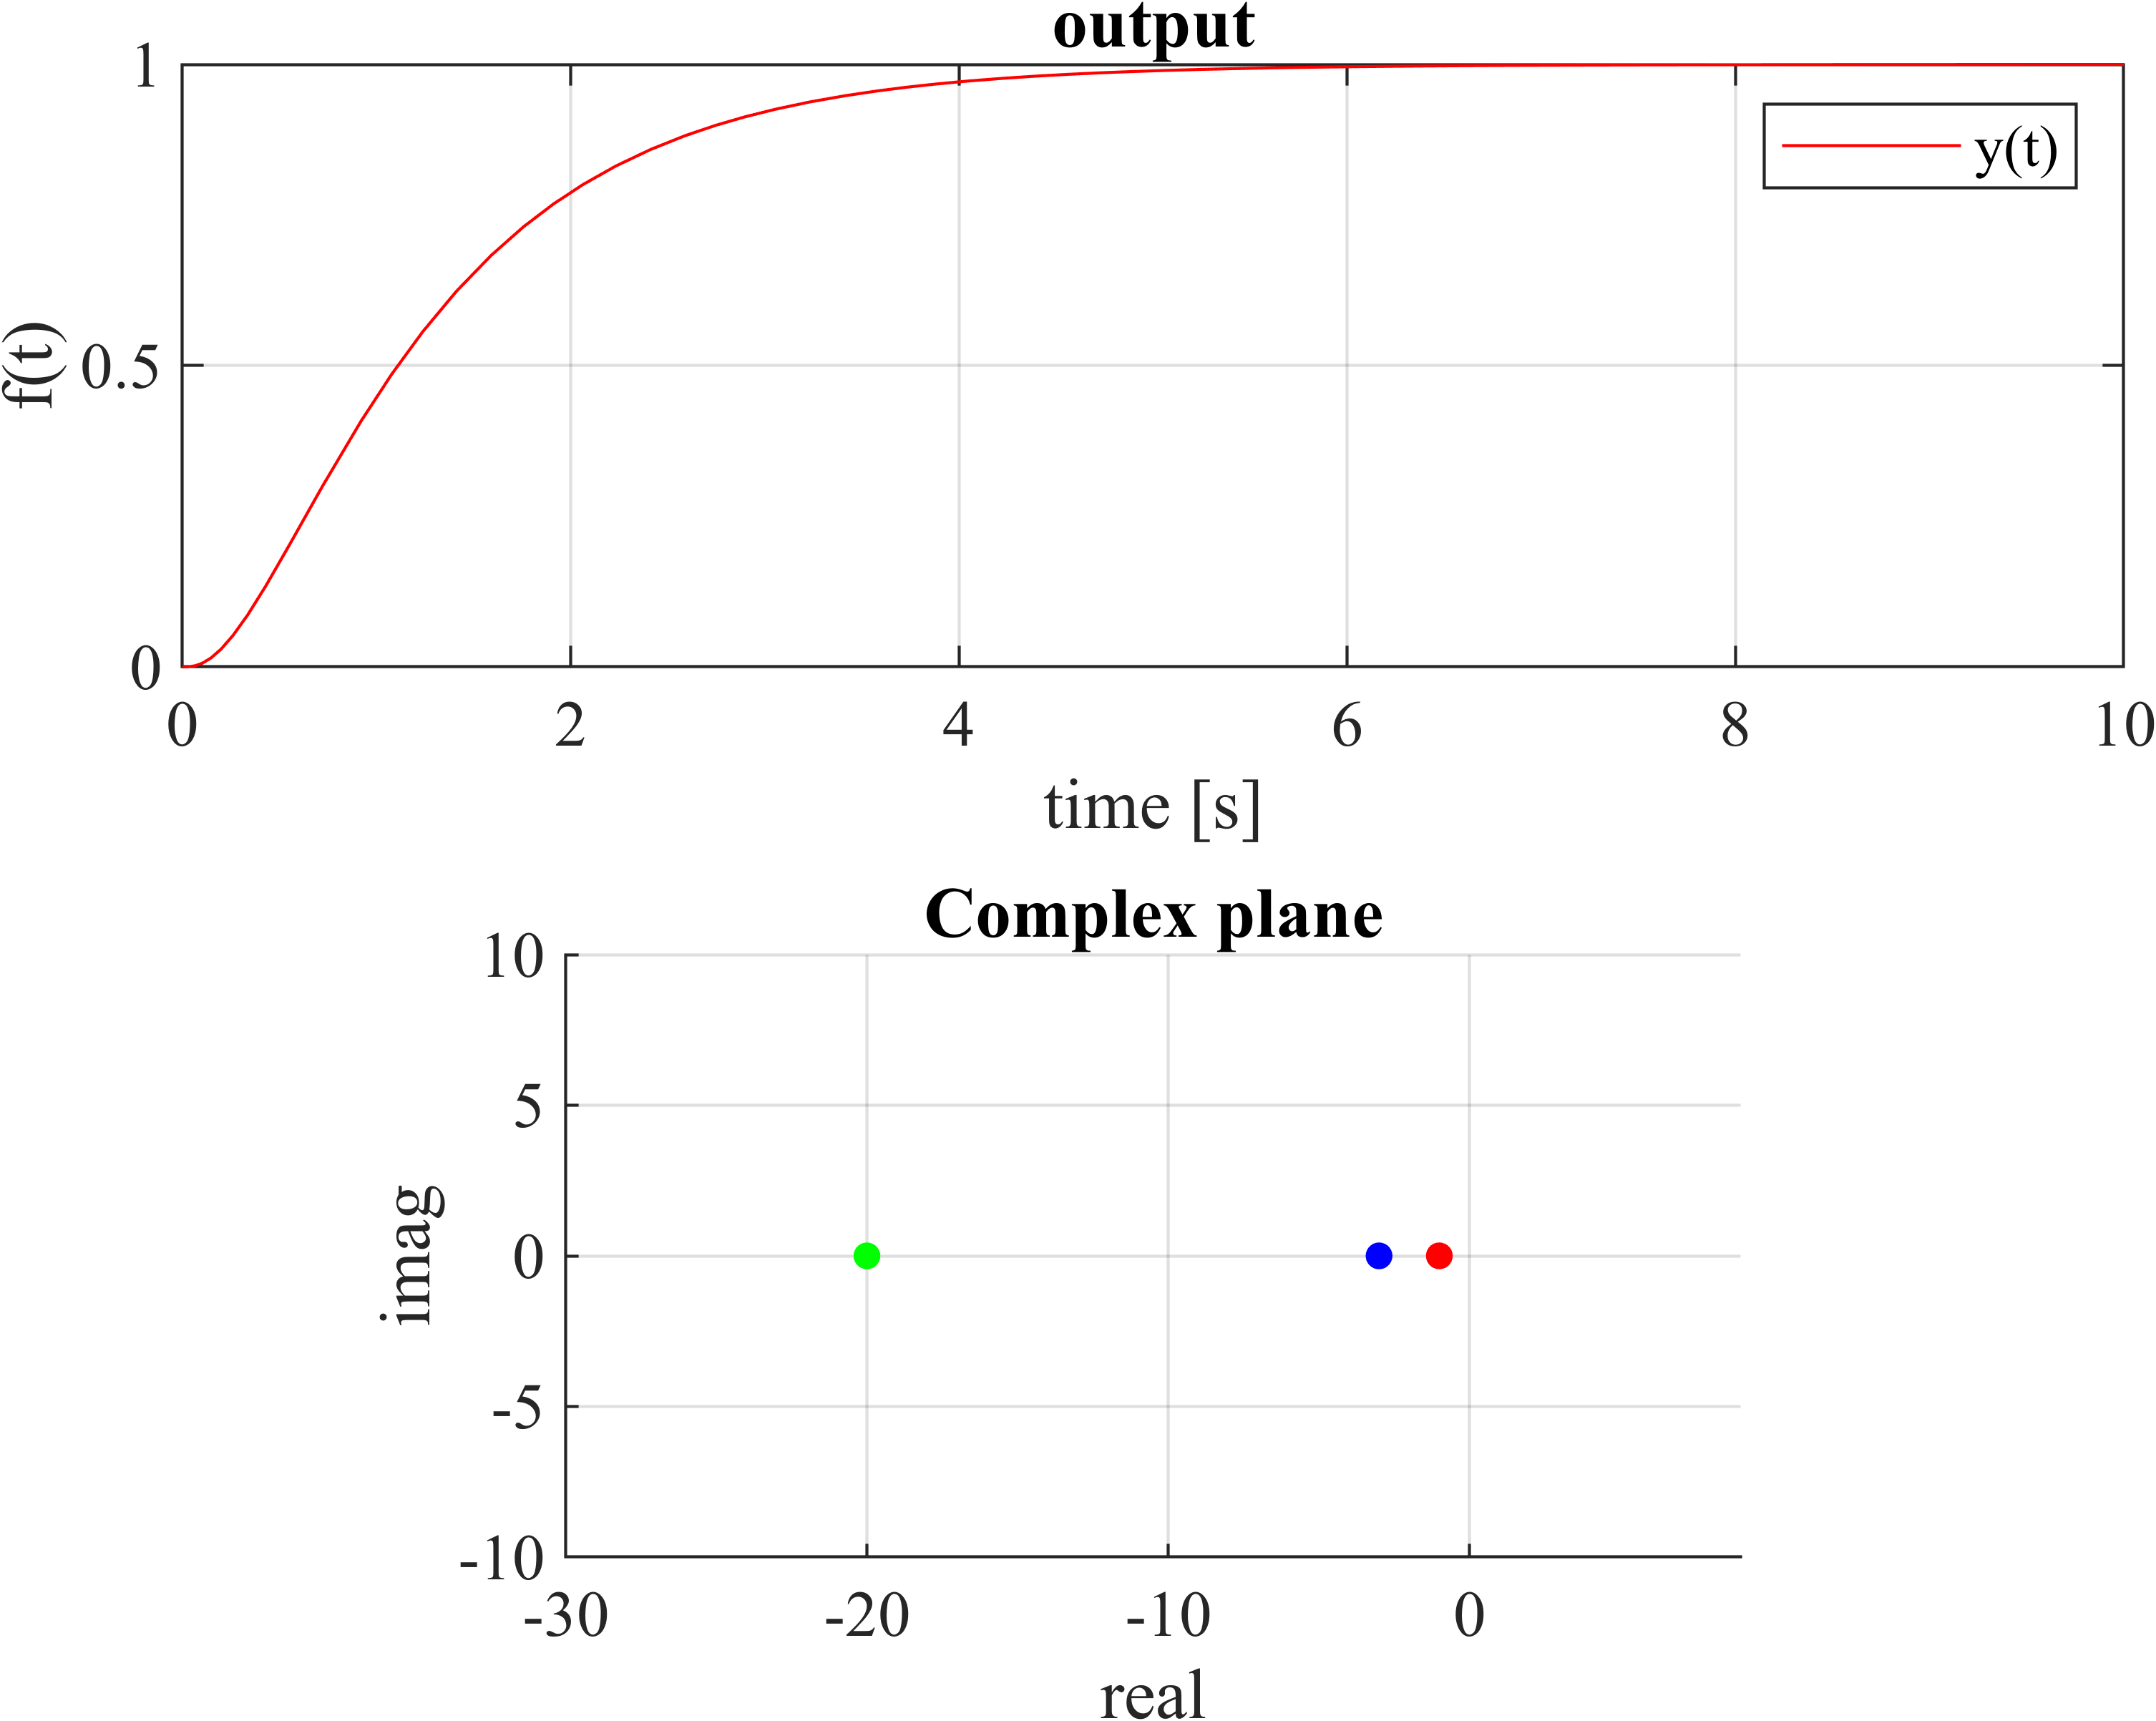
\includegraphics[width=0.8\textwidth]{output_task2_exp4.png}
  \caption{Симуляция - при $\lambda_1 = -1, \lambda_2 = -20,\lambda_3 = -3$}
\end{figure}
Получаем:
$$
\begin{aligned}
  \sigma_4 \approx 0\% \\
  t_4 \approx 4.4s
\end{aligned}
$$

\newpage
\section{5-й эксперимент}
\begin{figure}[ht]
    \centering
    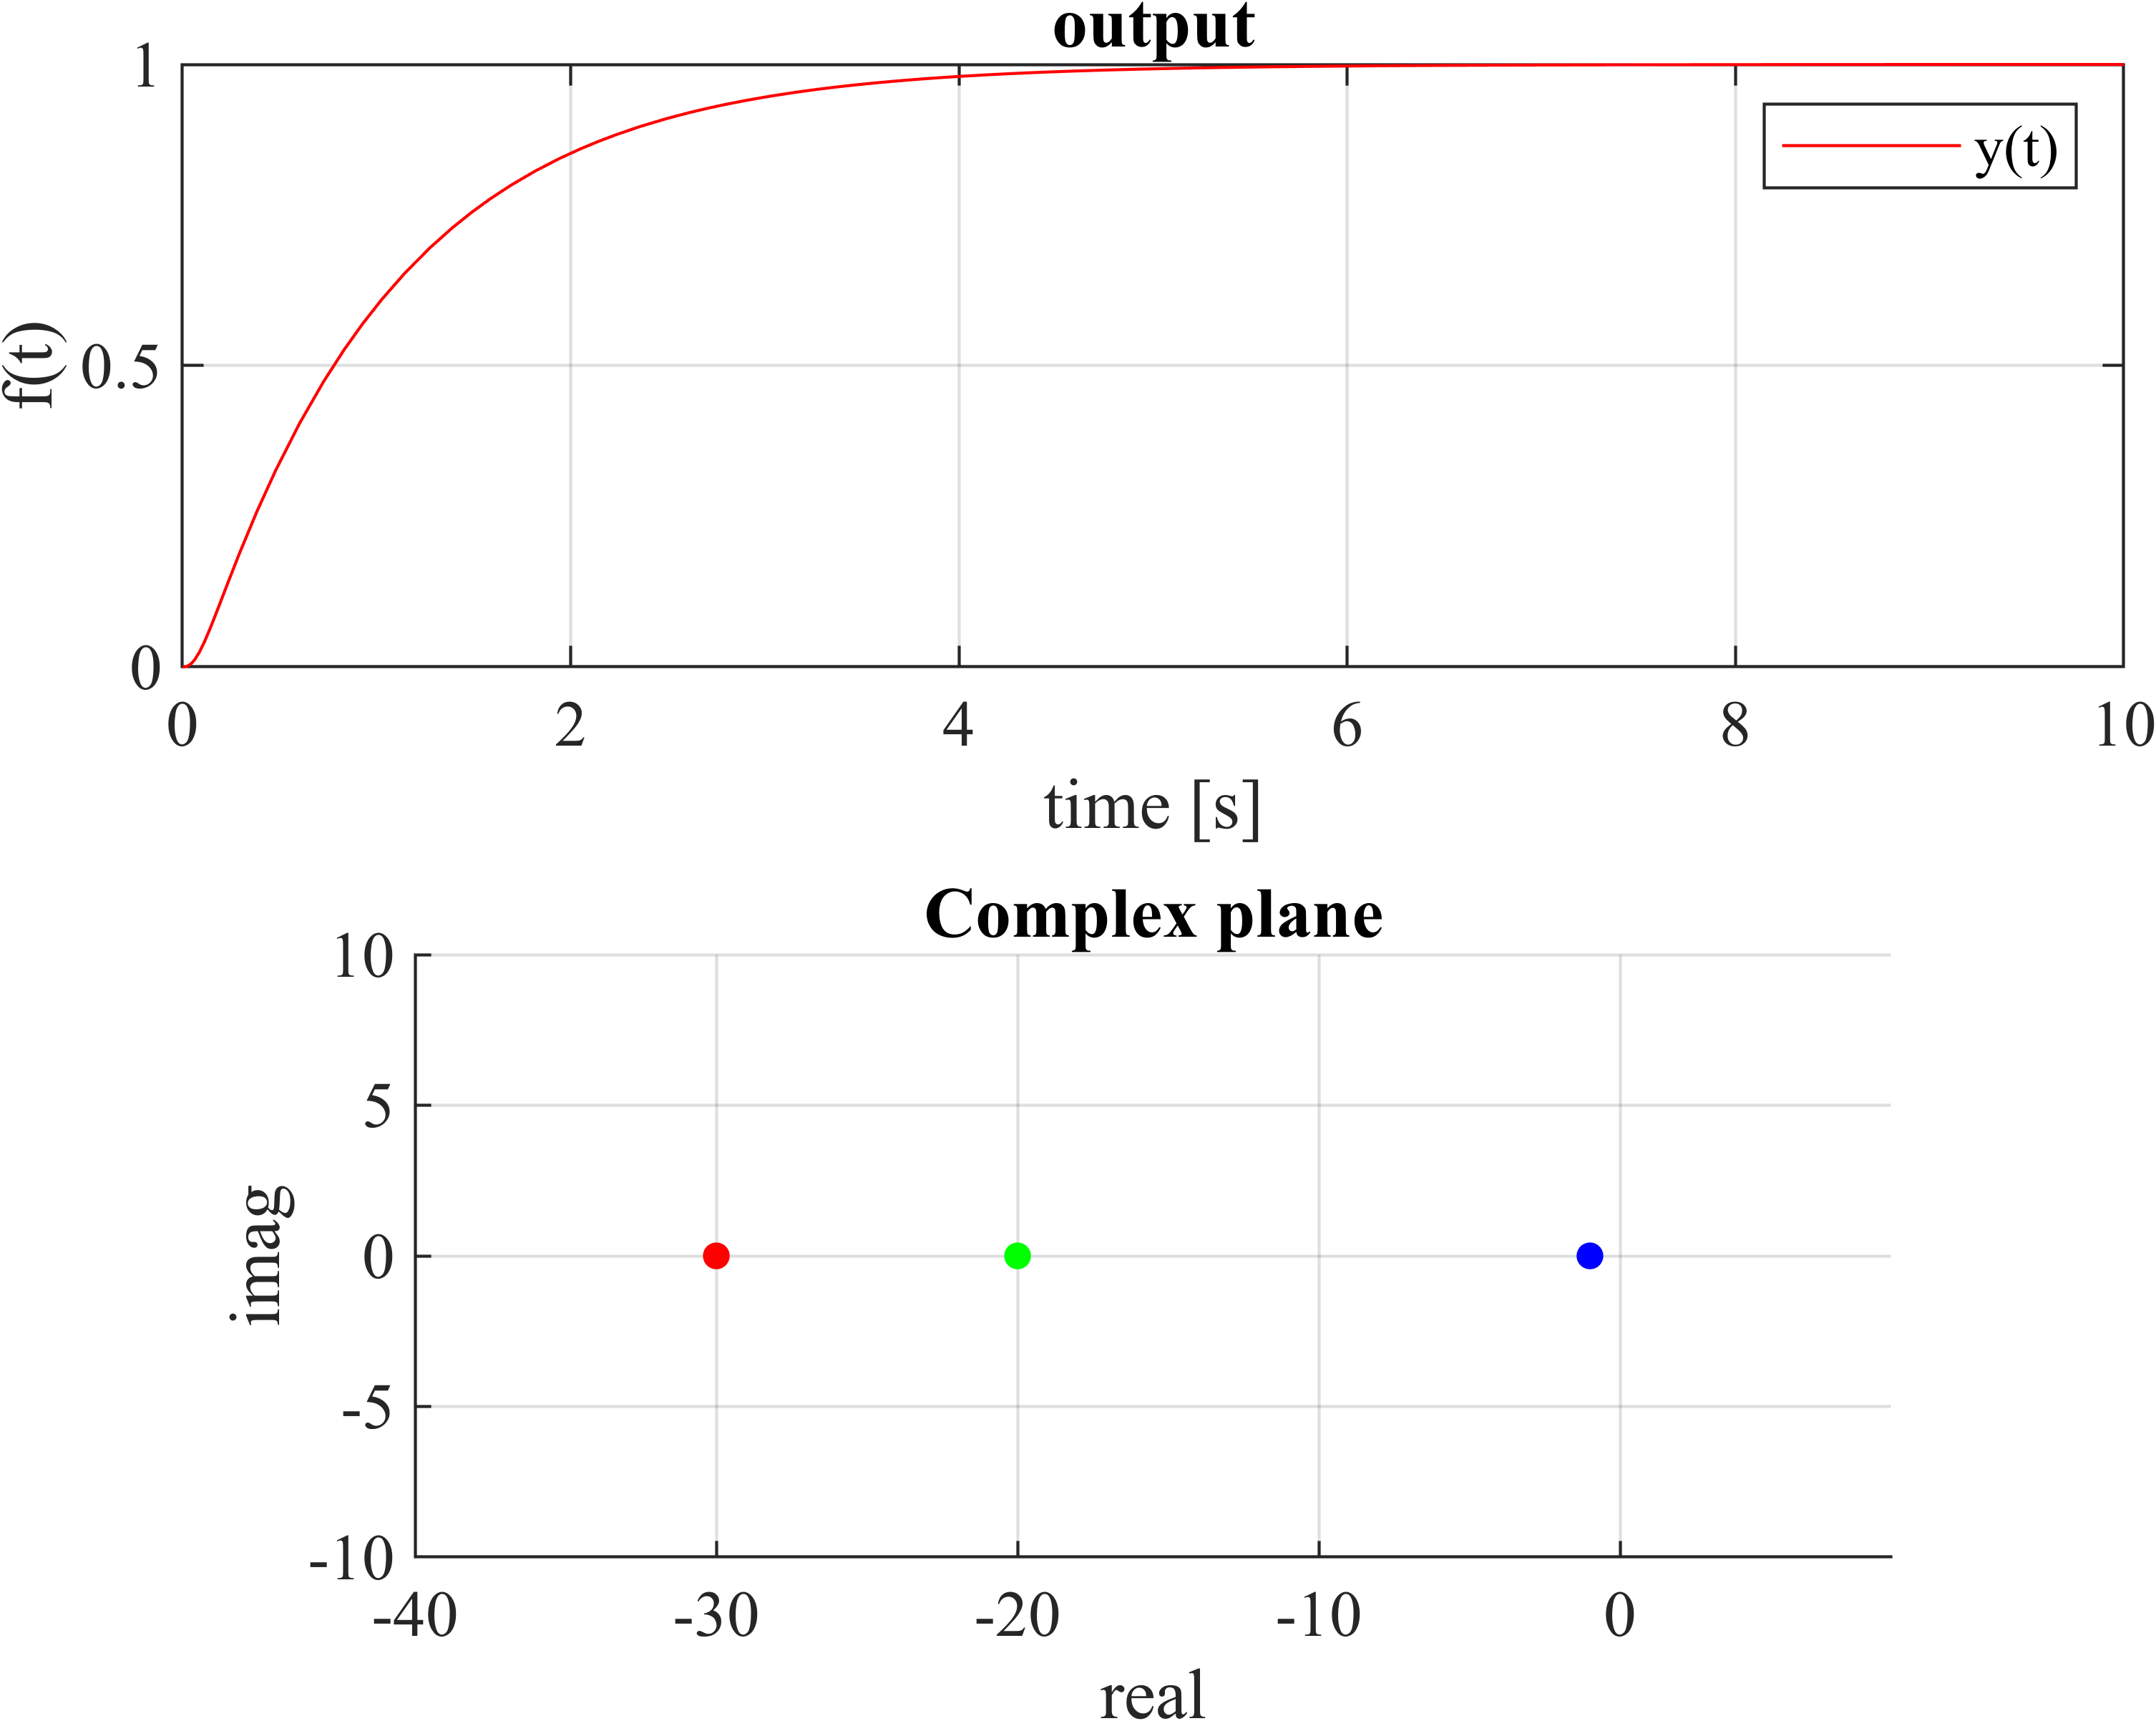
\includegraphics[width=0.8\textwidth]{output_task2_exp5.png}
  \caption{Симуляция - при $\lambda_1 = -30, \lambda_2 = -20,\lambda_3 = -1$}
\end{figure}
Получаем:
$$
\begin{aligned}
  \sigma_5 \approx 0\% \\
  t_5 \approx 4.0s
\end{aligned}
$$

\newpage
\section{6-й эксперимент}
\begin{figure}[ht]
    \centering
    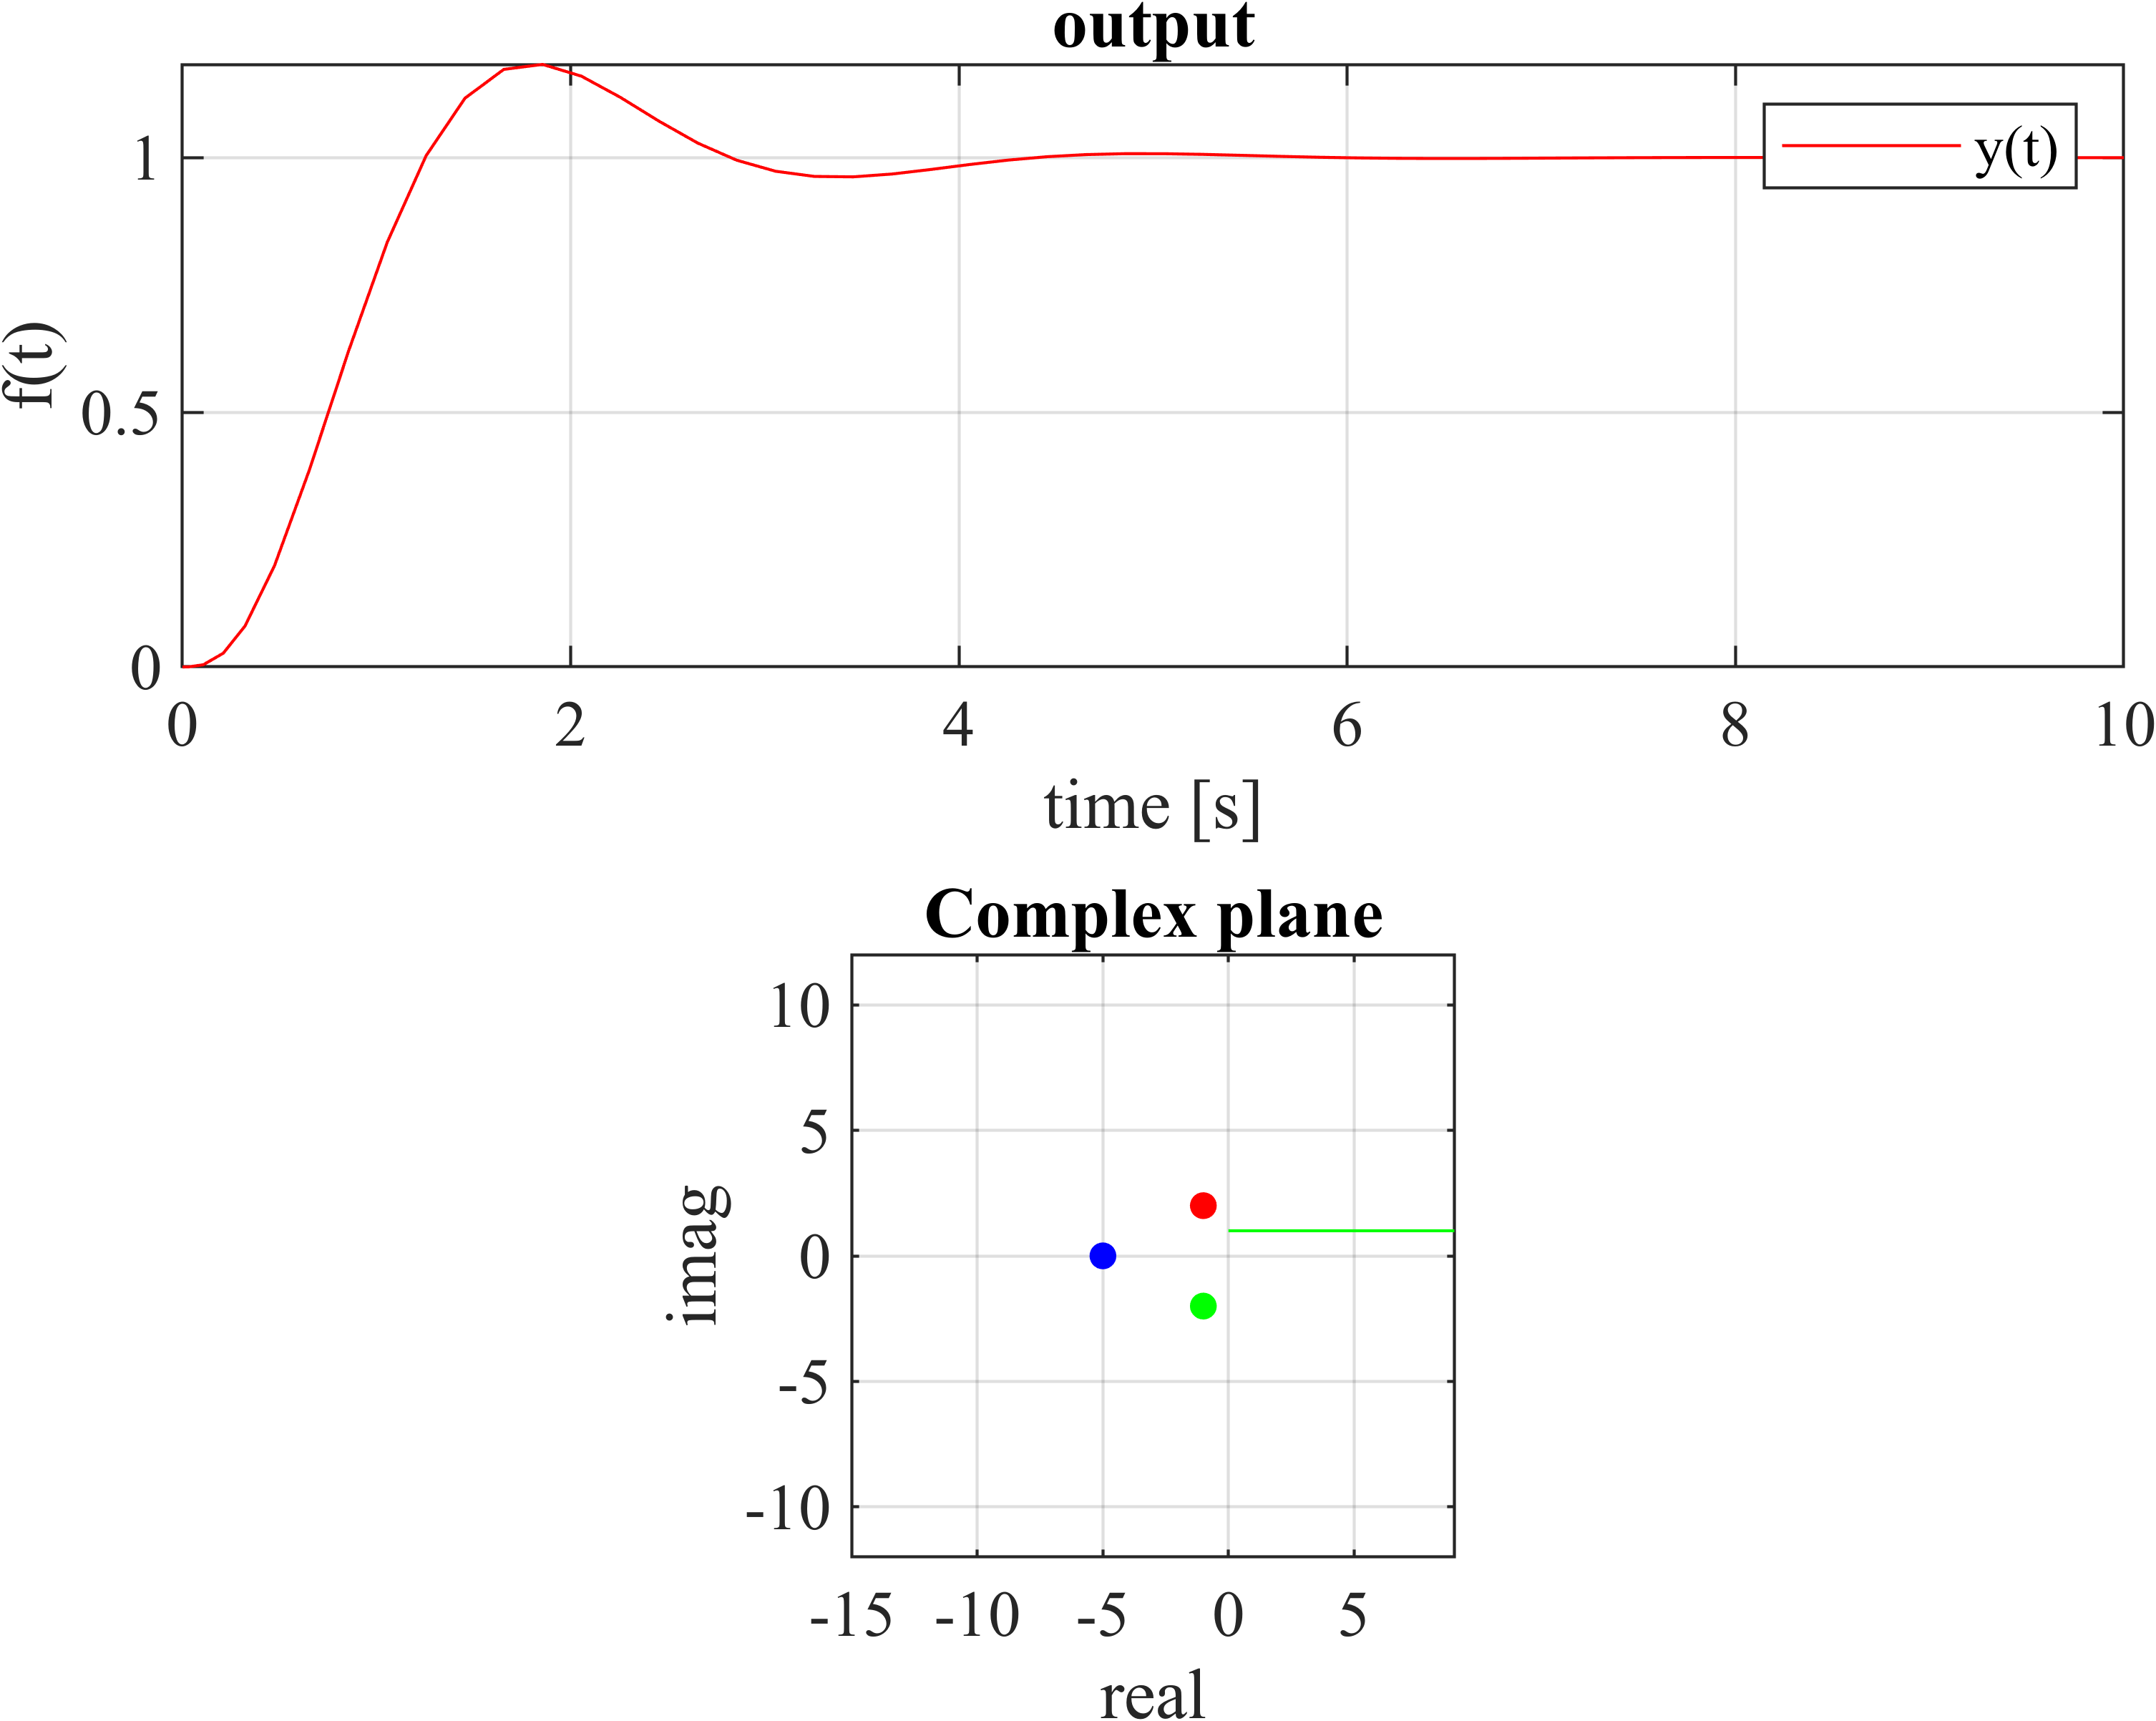
\includegraphics[width=0.8\textwidth]{output_task2_exp6.png}
  \caption{Симуляция - при $\lambda_1 = -1 + 2i, \lambda_2 = -1 -2i,\lambda_3 = -5$}
\end{figure}
Получаем:
$$
\begin{aligned}
  \sigma_6 \approx 18\% \\
  t_6 \approx 4.2s
\end{aligned}
$$
Даже больше, думаю не совсем корректно говорить о времени переходного процесса в данном случае, потому что процесс циклический.

\newpage
\section{7-й эксперимент}
\begin{figure}[ht]
    \centering
    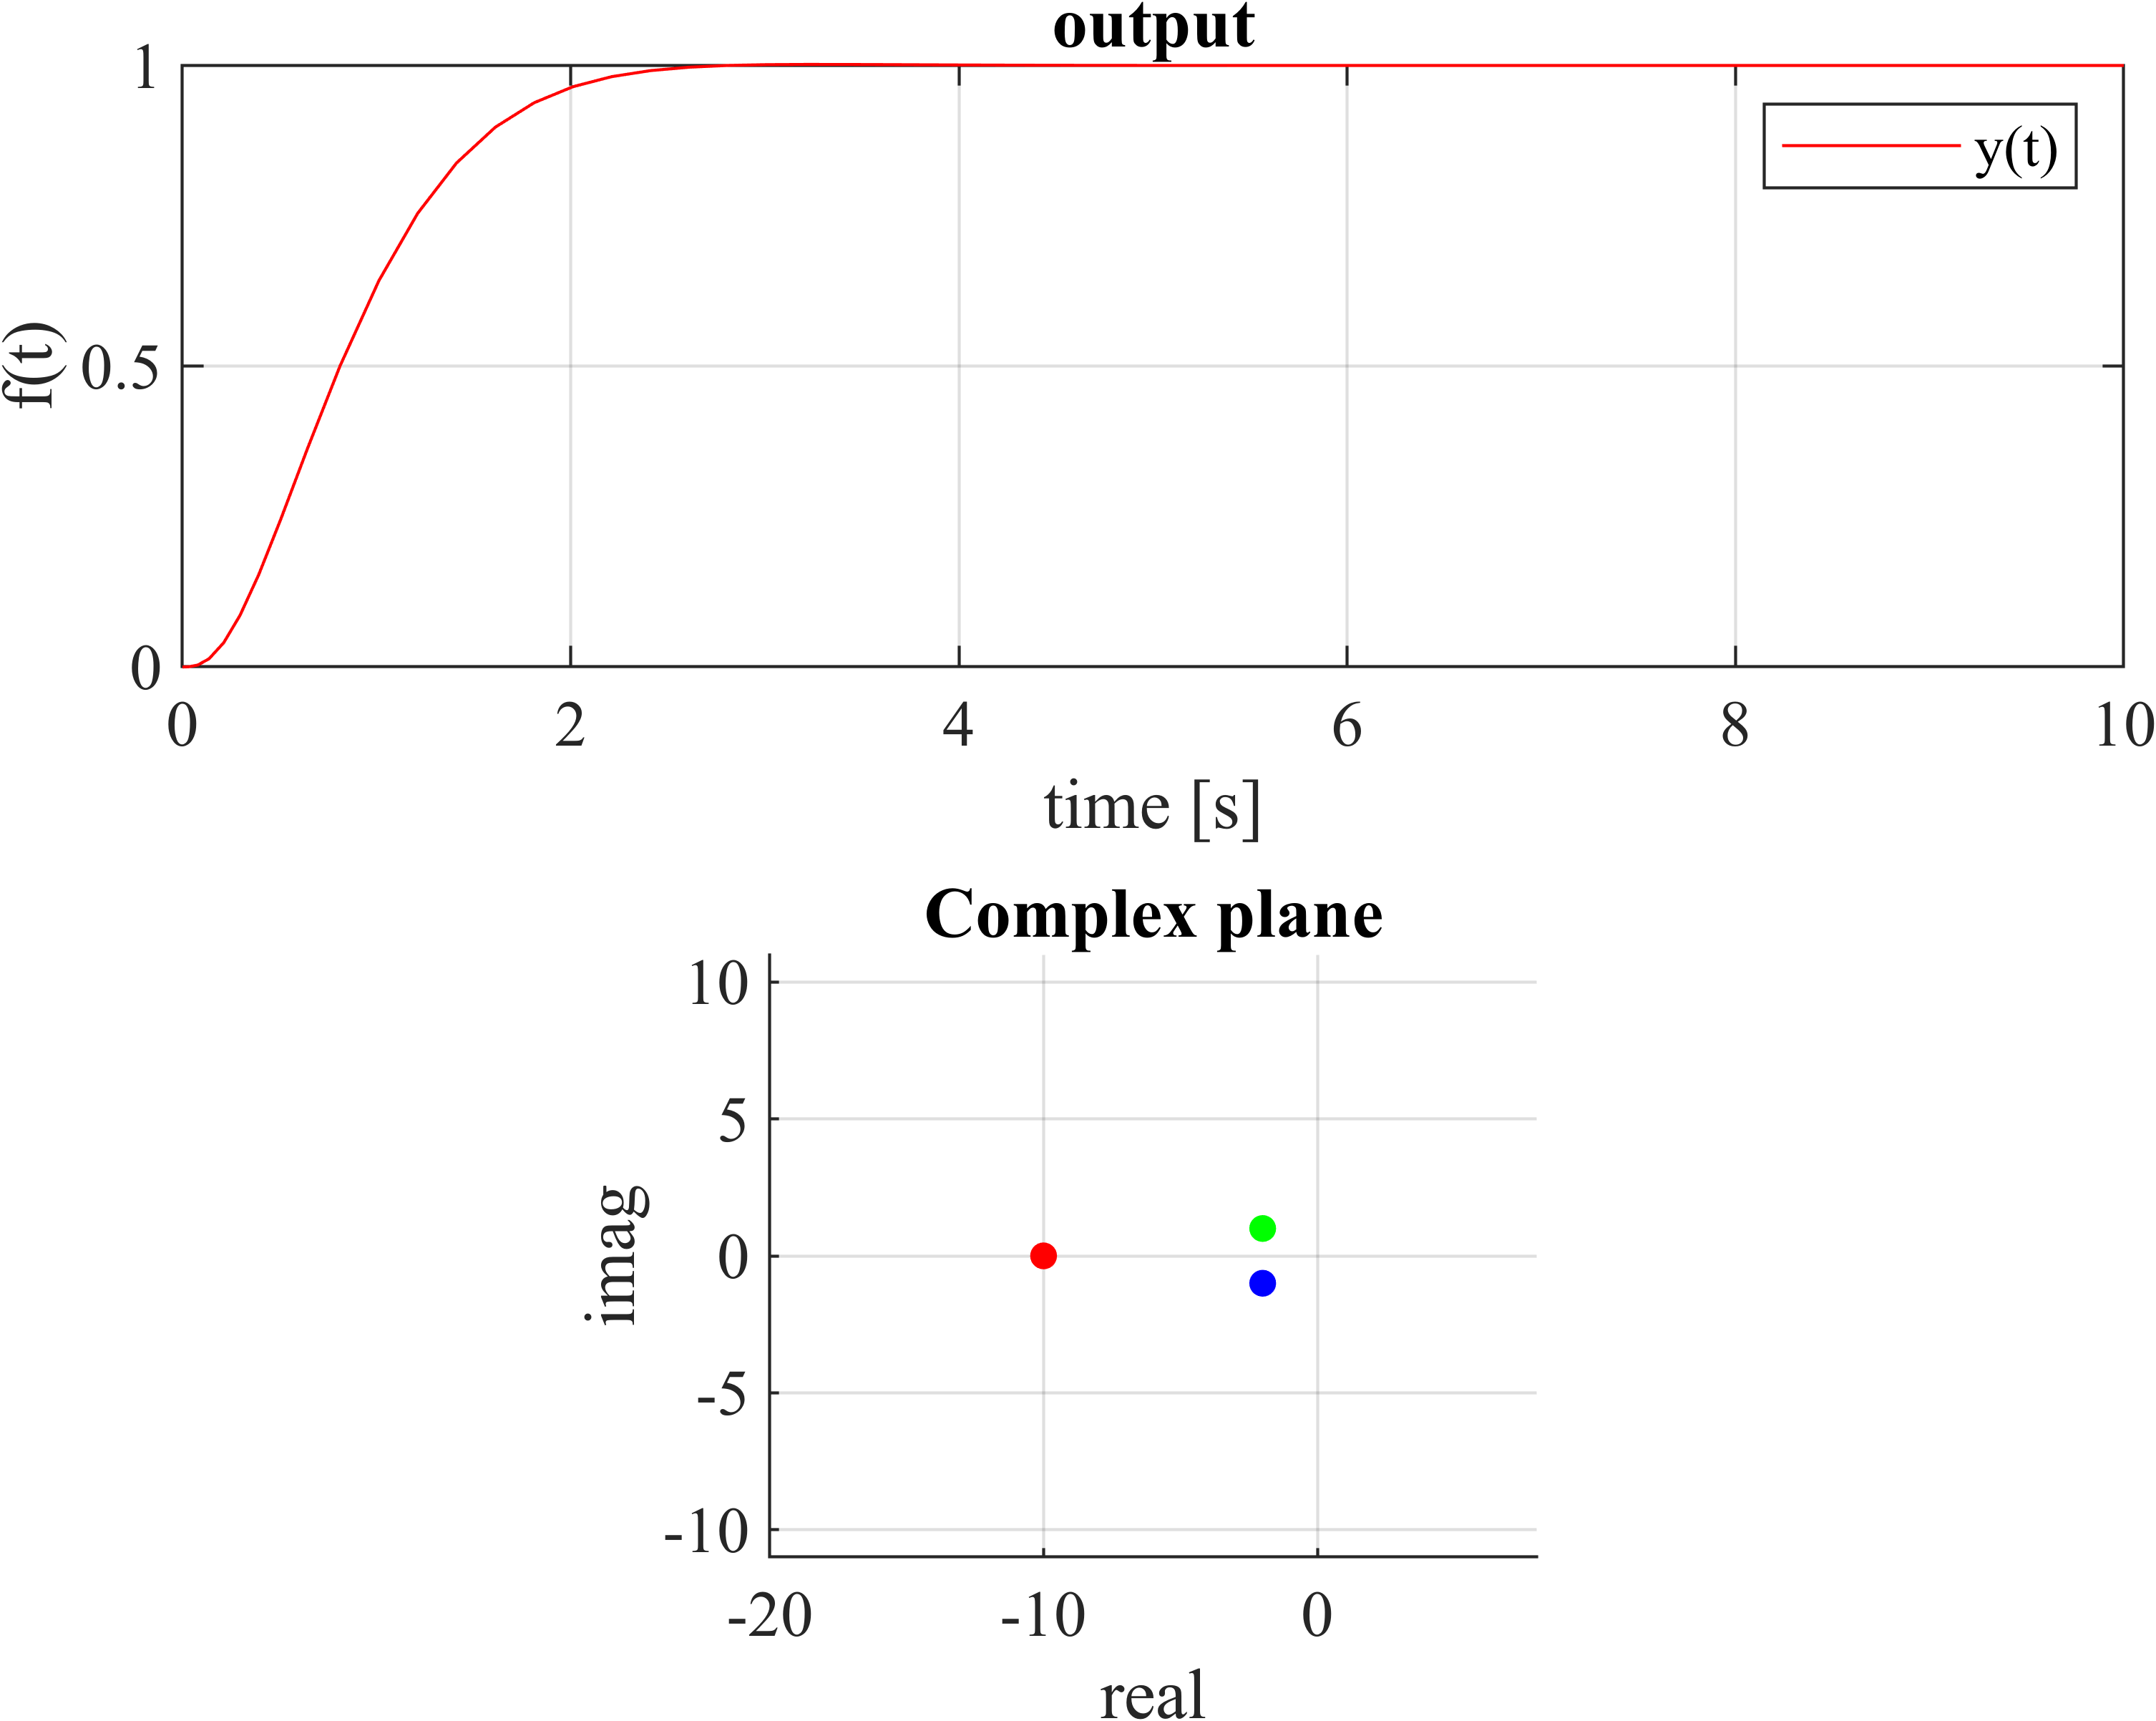
\includegraphics[width=0.8\textwidth]{output_task2_exp7.png}
  \caption{Симуляция - при $\lambda_1 = -10, \lambda_2 = -2 + i,\lambda_3 = -2 - i$}
\end{figure}
Получаем:
$$
\begin{aligned}
  \sigma_7 \approx 0.1\% \\
  t_7 \approx 2.2s
\end{aligned}
$$

\newpage
\section{8-й эксперимент}
\begin{figure}[ht]
    \centering
    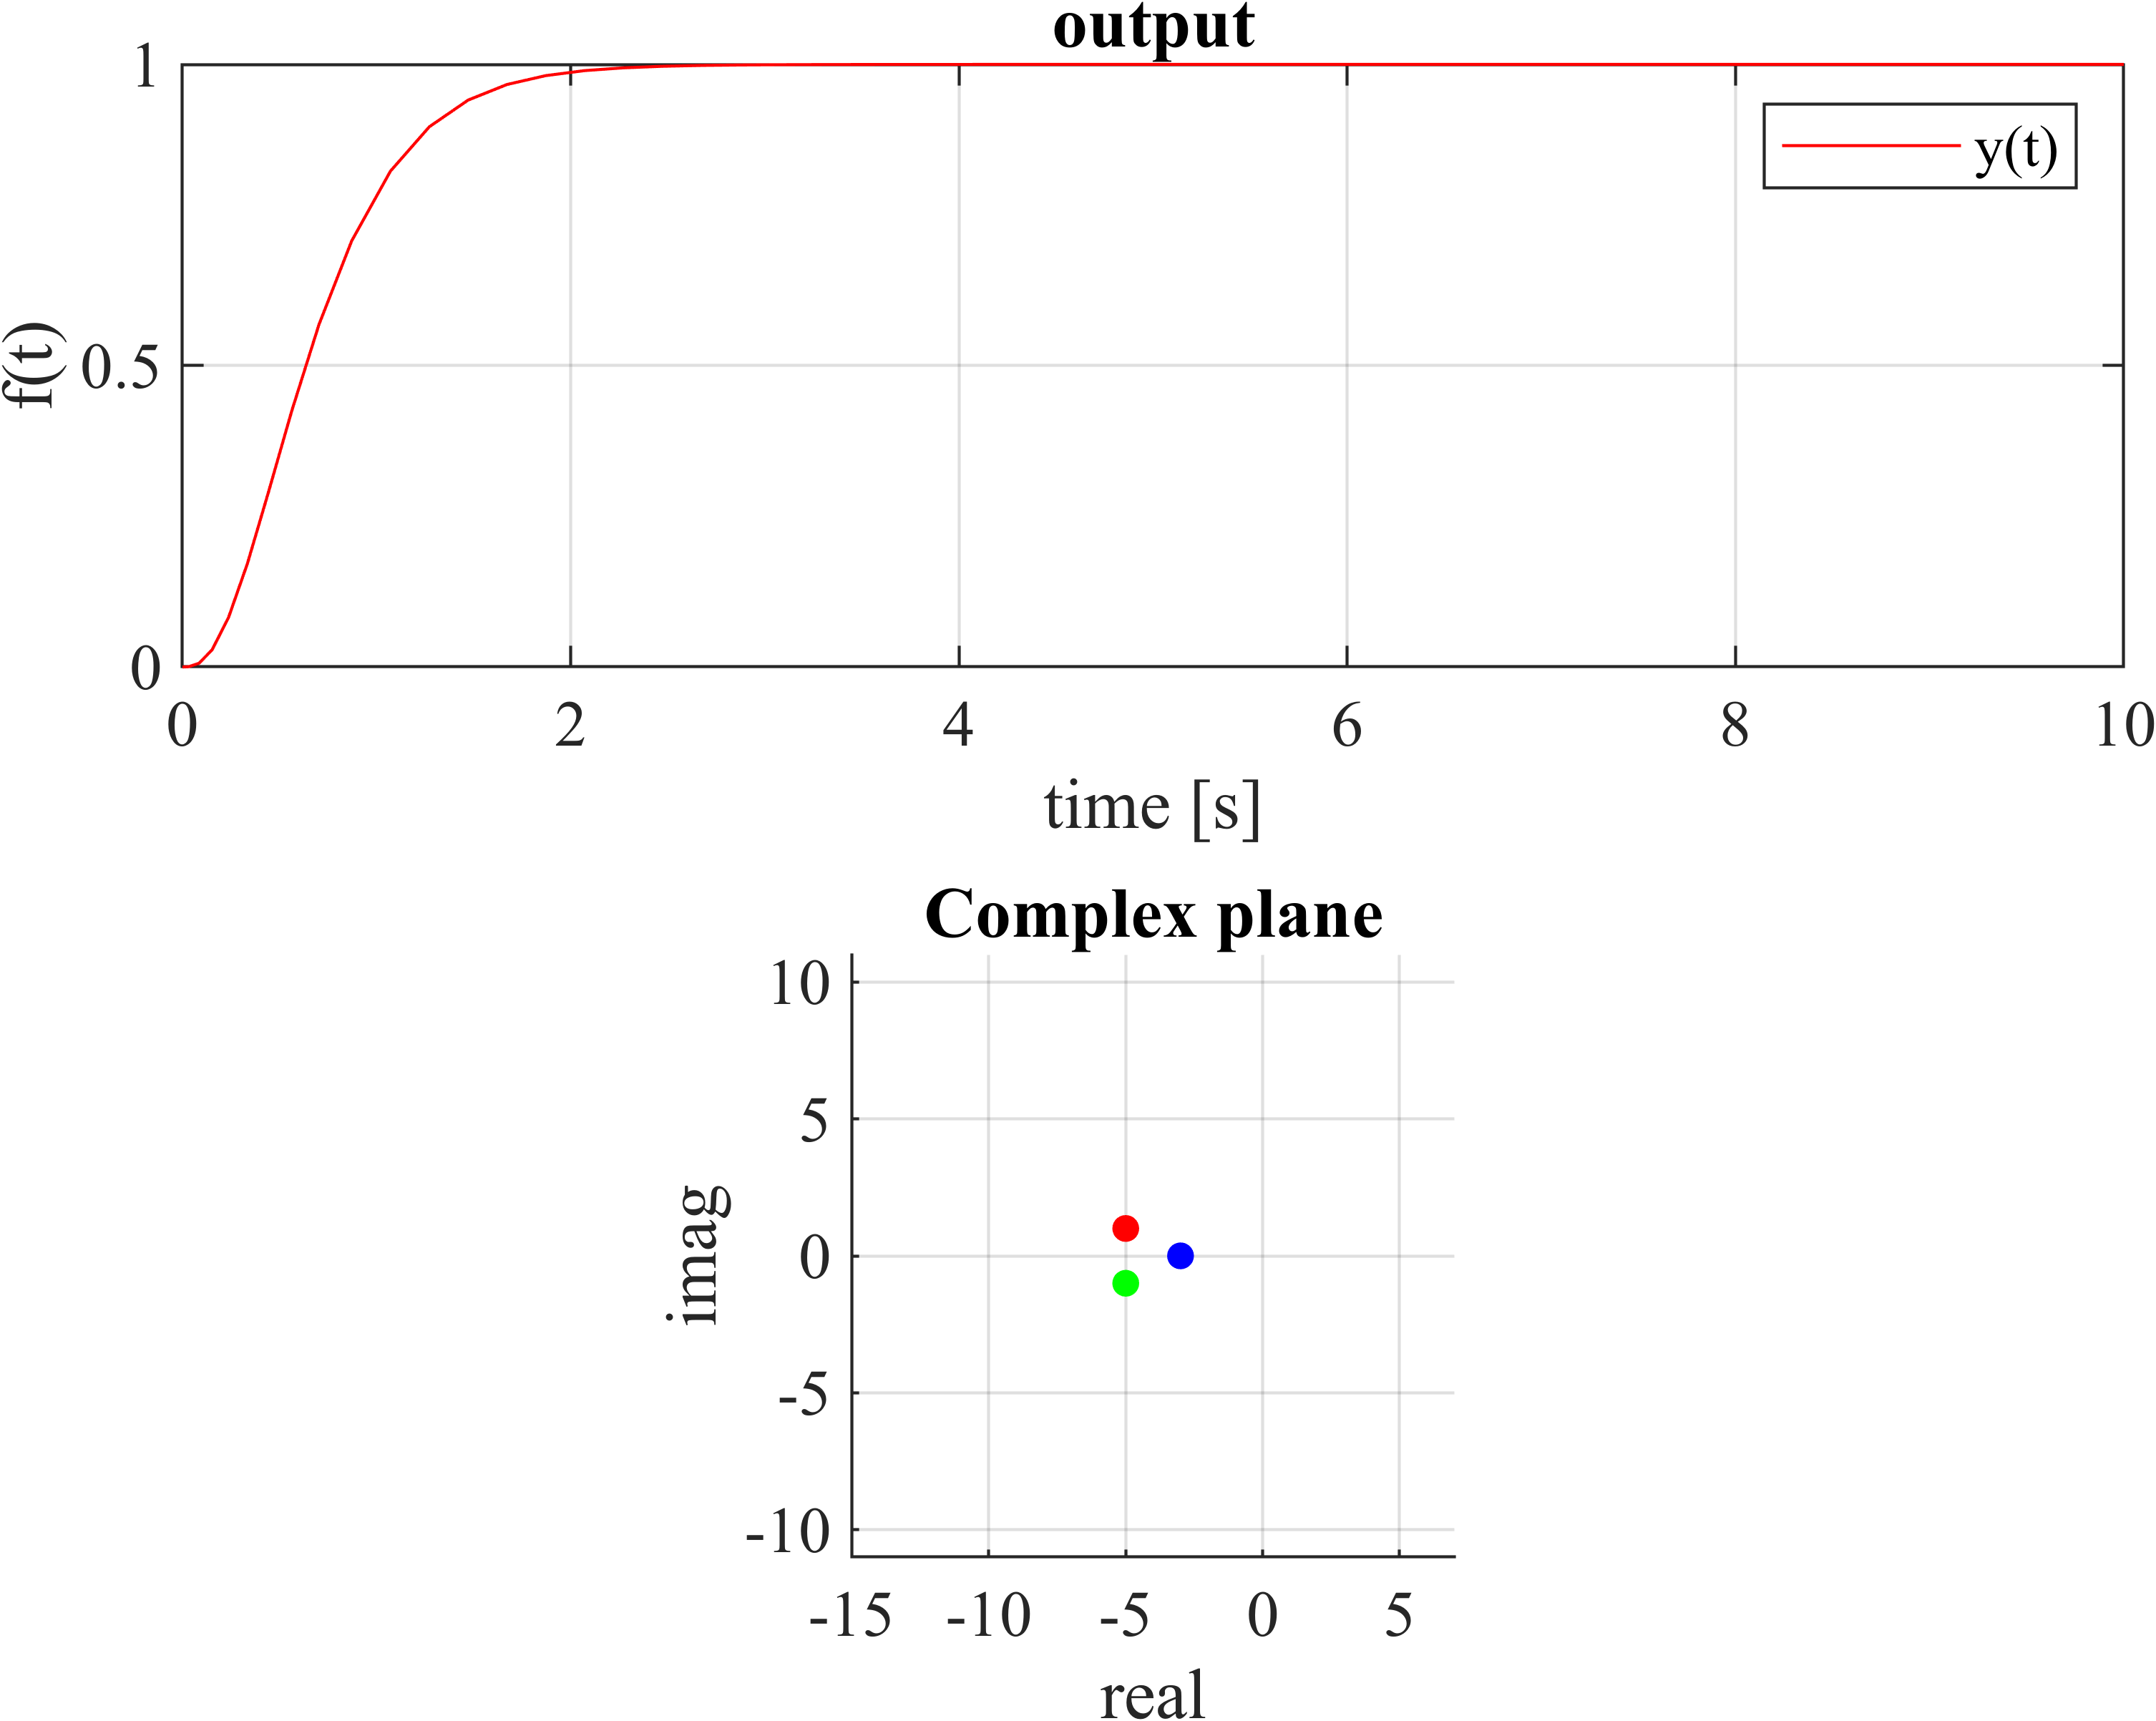
\includegraphics[width=0.8\textwidth]{output_task2_exp8.png}
  \caption{Симуляция - при $\lambda_1 = -5 + i, \lambda_2 = -5 - i,\lambda_3 = -3$}
\end{figure}
Получаем:
$$
\begin{aligned}
  \sigma_8 \approx 0\% \\
  t_8 \approx 1.8s
\end{aligned}
$$

\newpage
\section{9-й эксперимент}
\begin{figure}[ht]
    \centering
    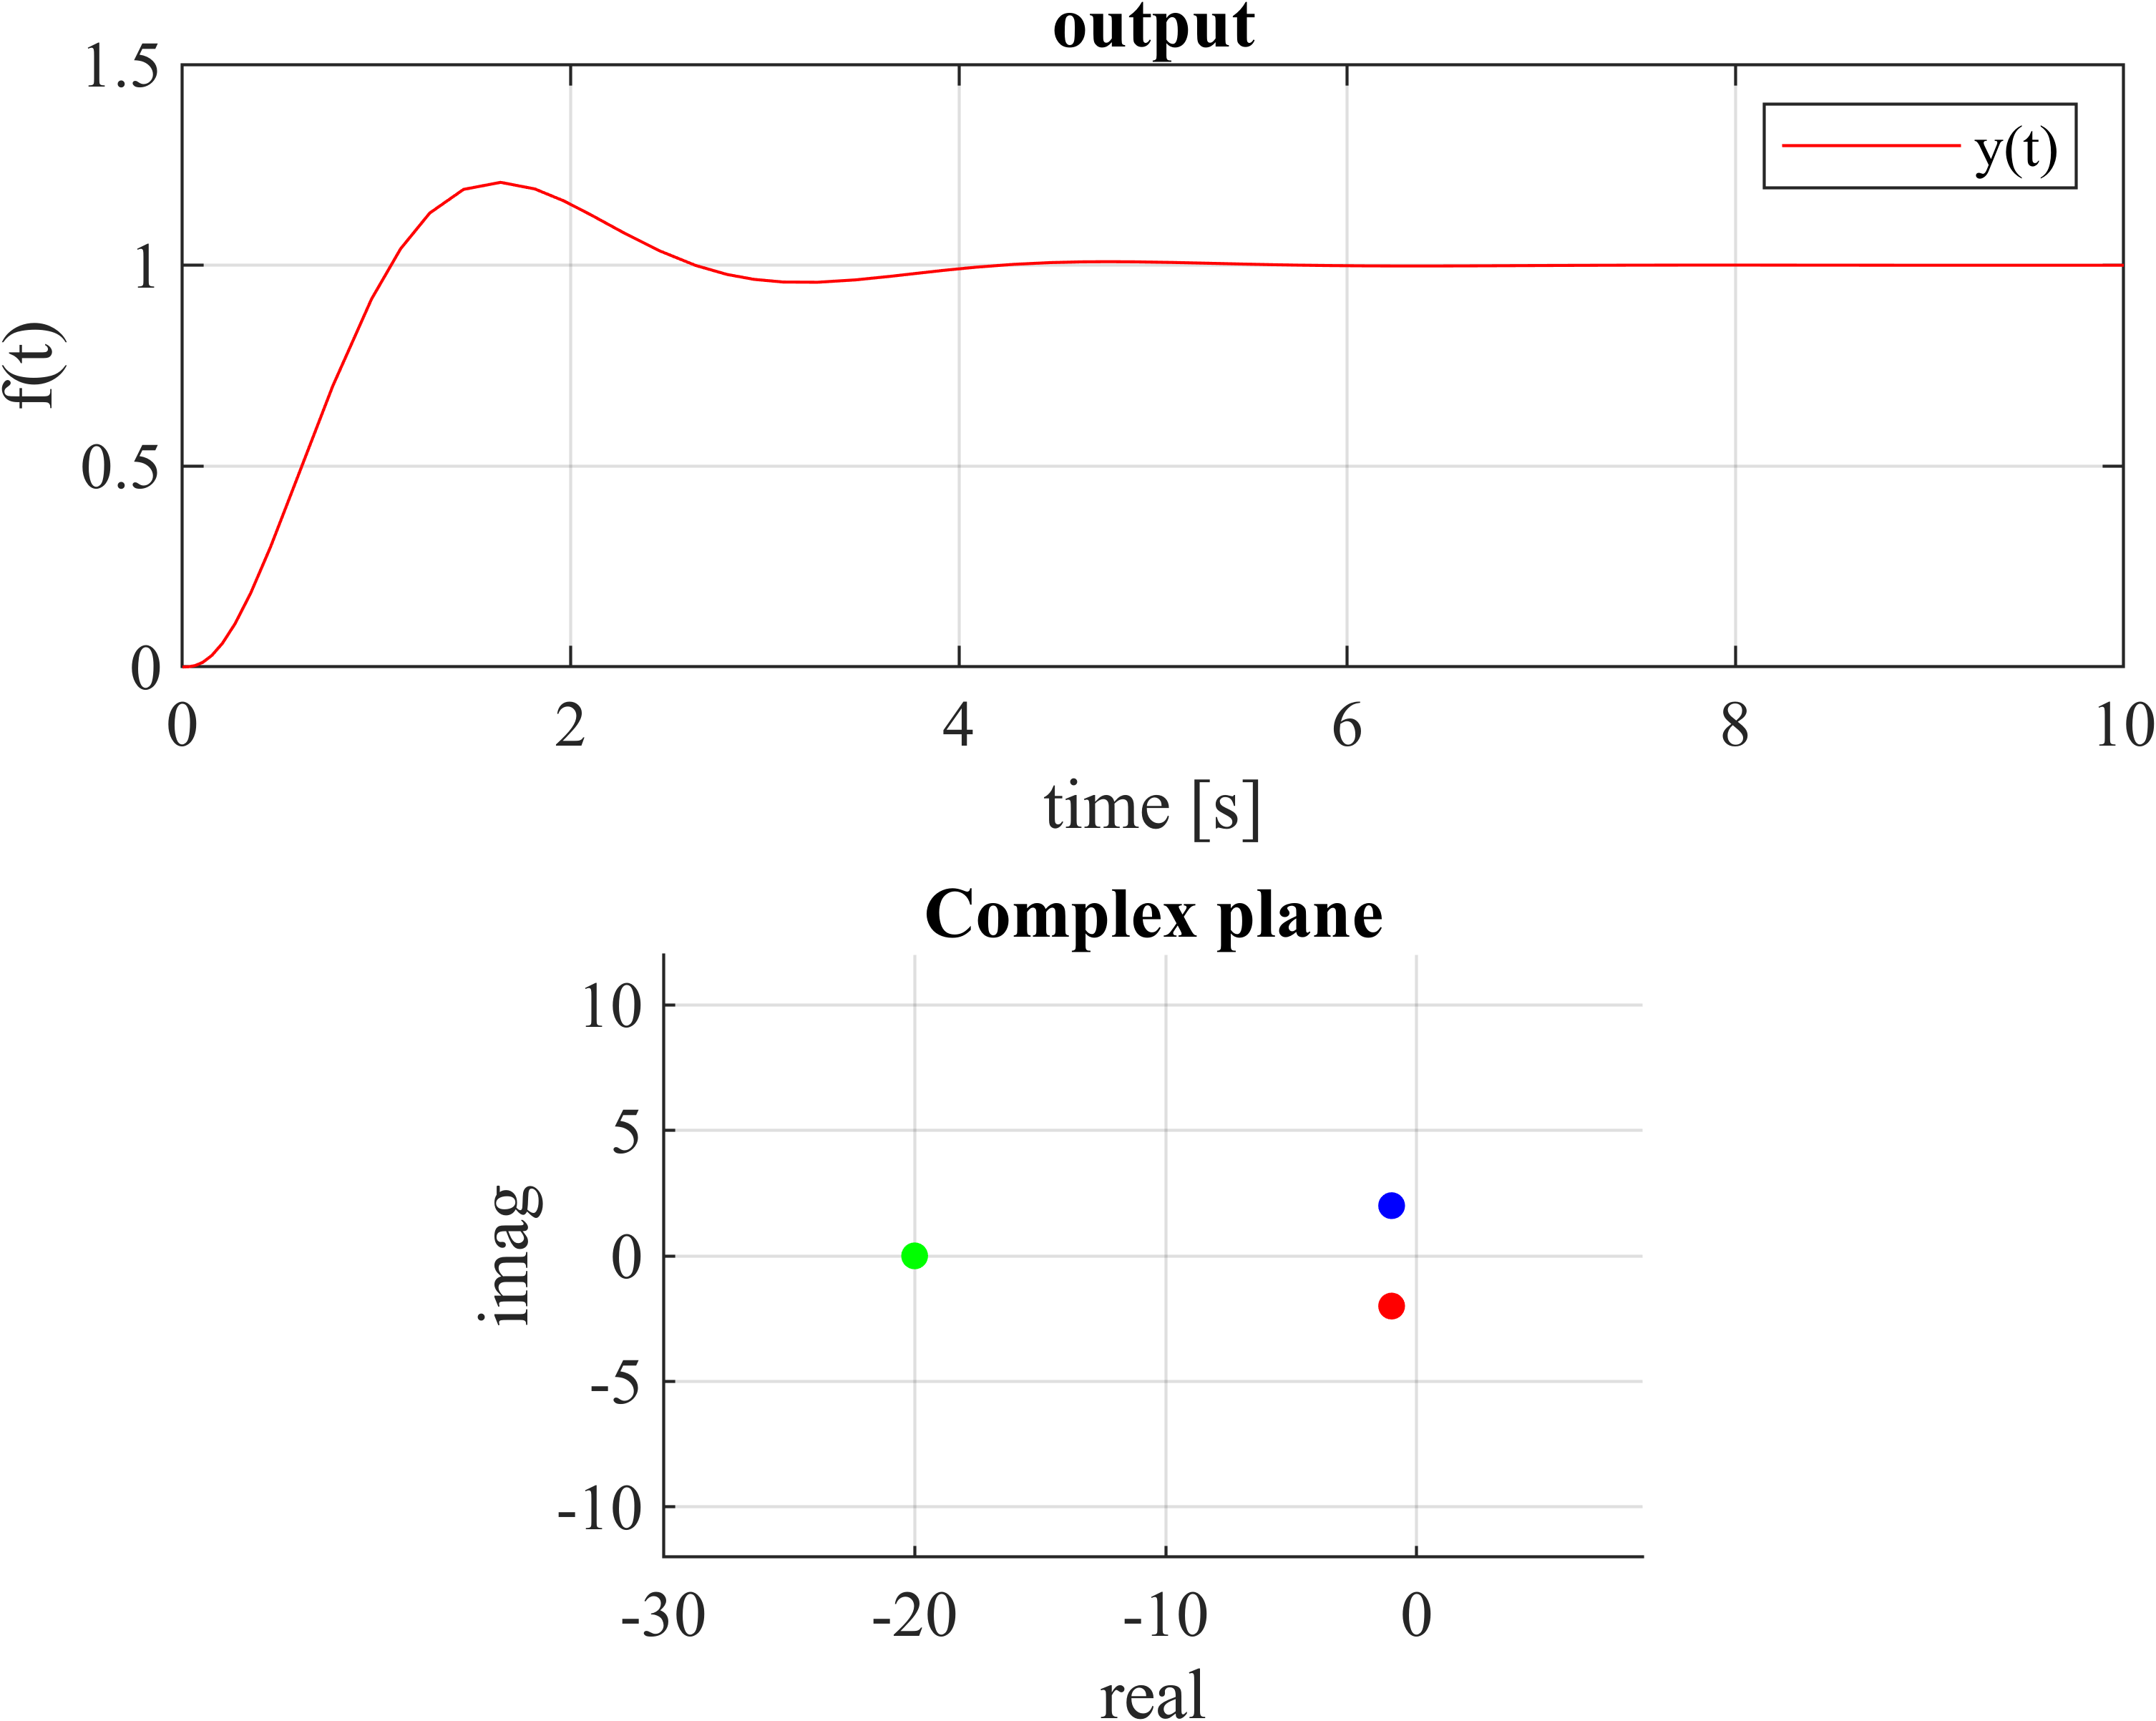
\includegraphics[width=0.8\textwidth]{output_task2_exp9.png}
  \caption{Симуляция - при $\lambda_1 = -1 -2i, \lambda_2 = -1 +2i,\lambda_3 = -20$}
\end{figure}
Получаем:
$$
\begin{aligned}
  \sigma_9 \approx 20\% \\
  t_9 \approx 4.0s
\end{aligned}
$$

\newpage
\section{10-й эксперимент}
\begin{figure}[ht]
    \centering
    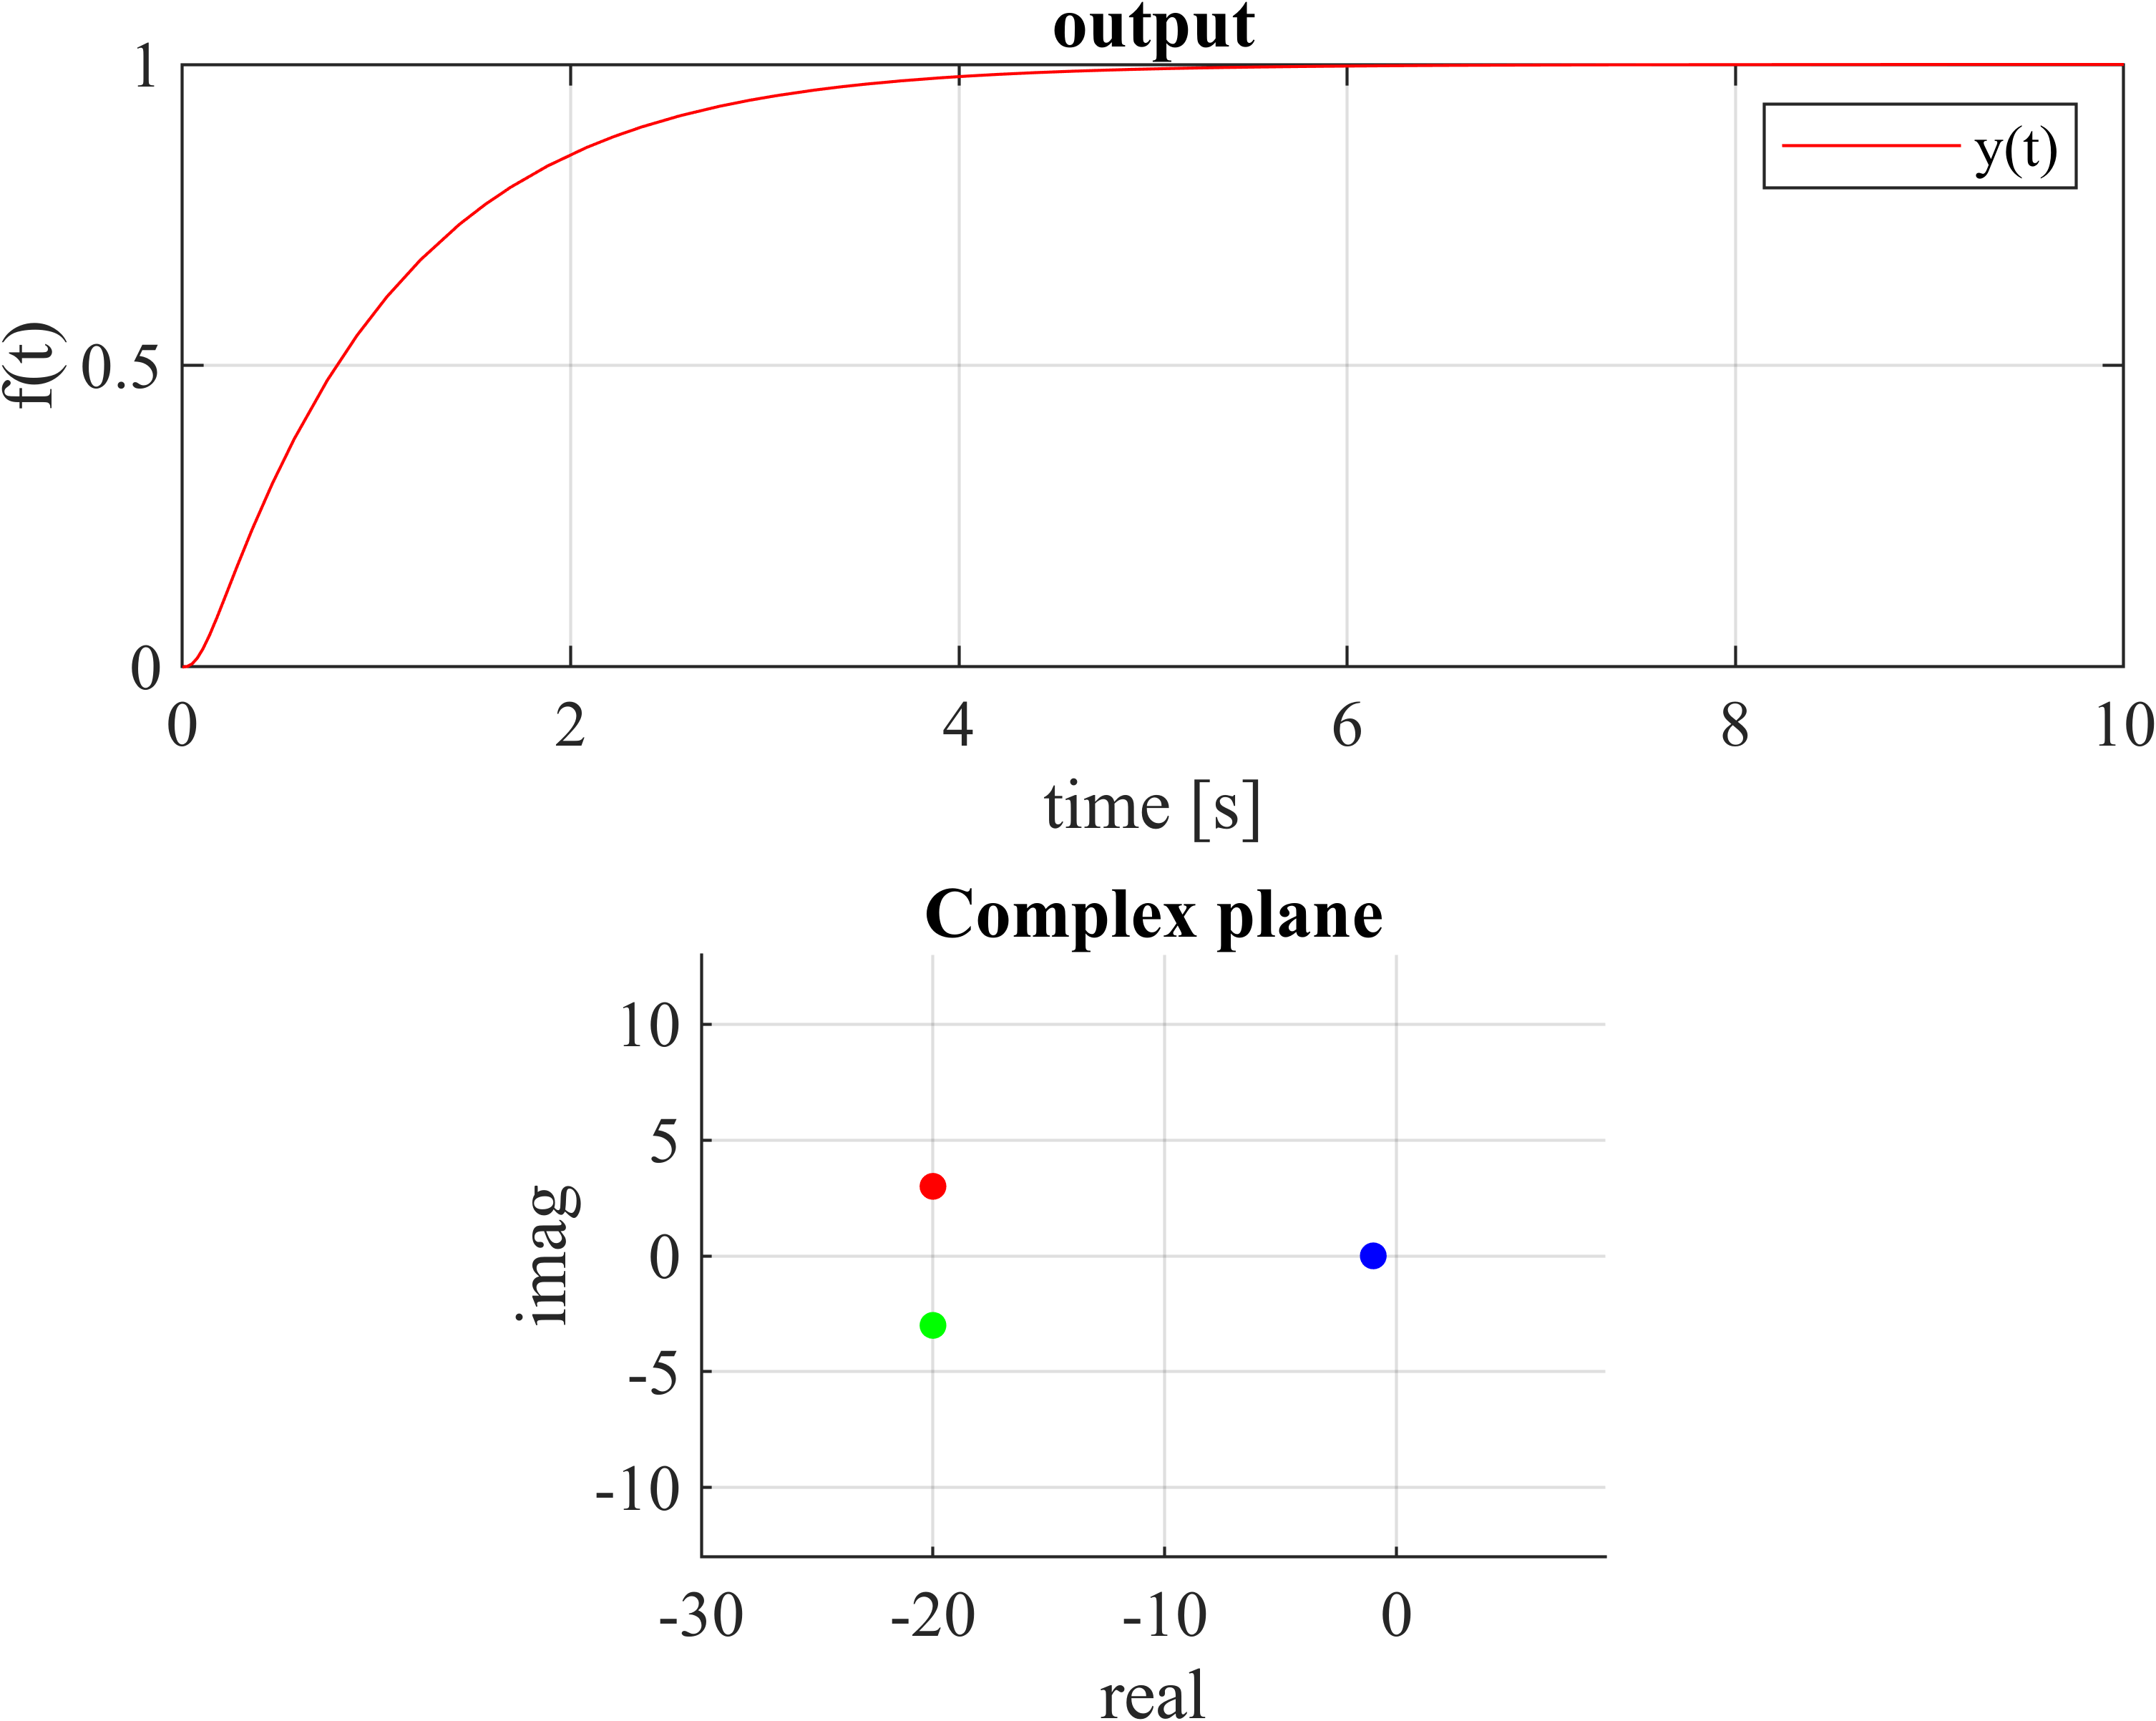
\includegraphics[width=0.8\textwidth]{output_task2_exp10.png}
  \caption{Симуляция - при $\lambda_1 = -20 +3i, \lambda_2 = -20 - 3i,\lambda_3 = -1$}
\end{figure}
Получаем:
$$
\begin{aligned}
  \sigma_{10} \approx 0\% \\
  t_{10} \approx 4.1s
\end{aligned}
$$

\newpage
\section{11-й эксперимент}
\begin{figure}[ht]
    \centering
    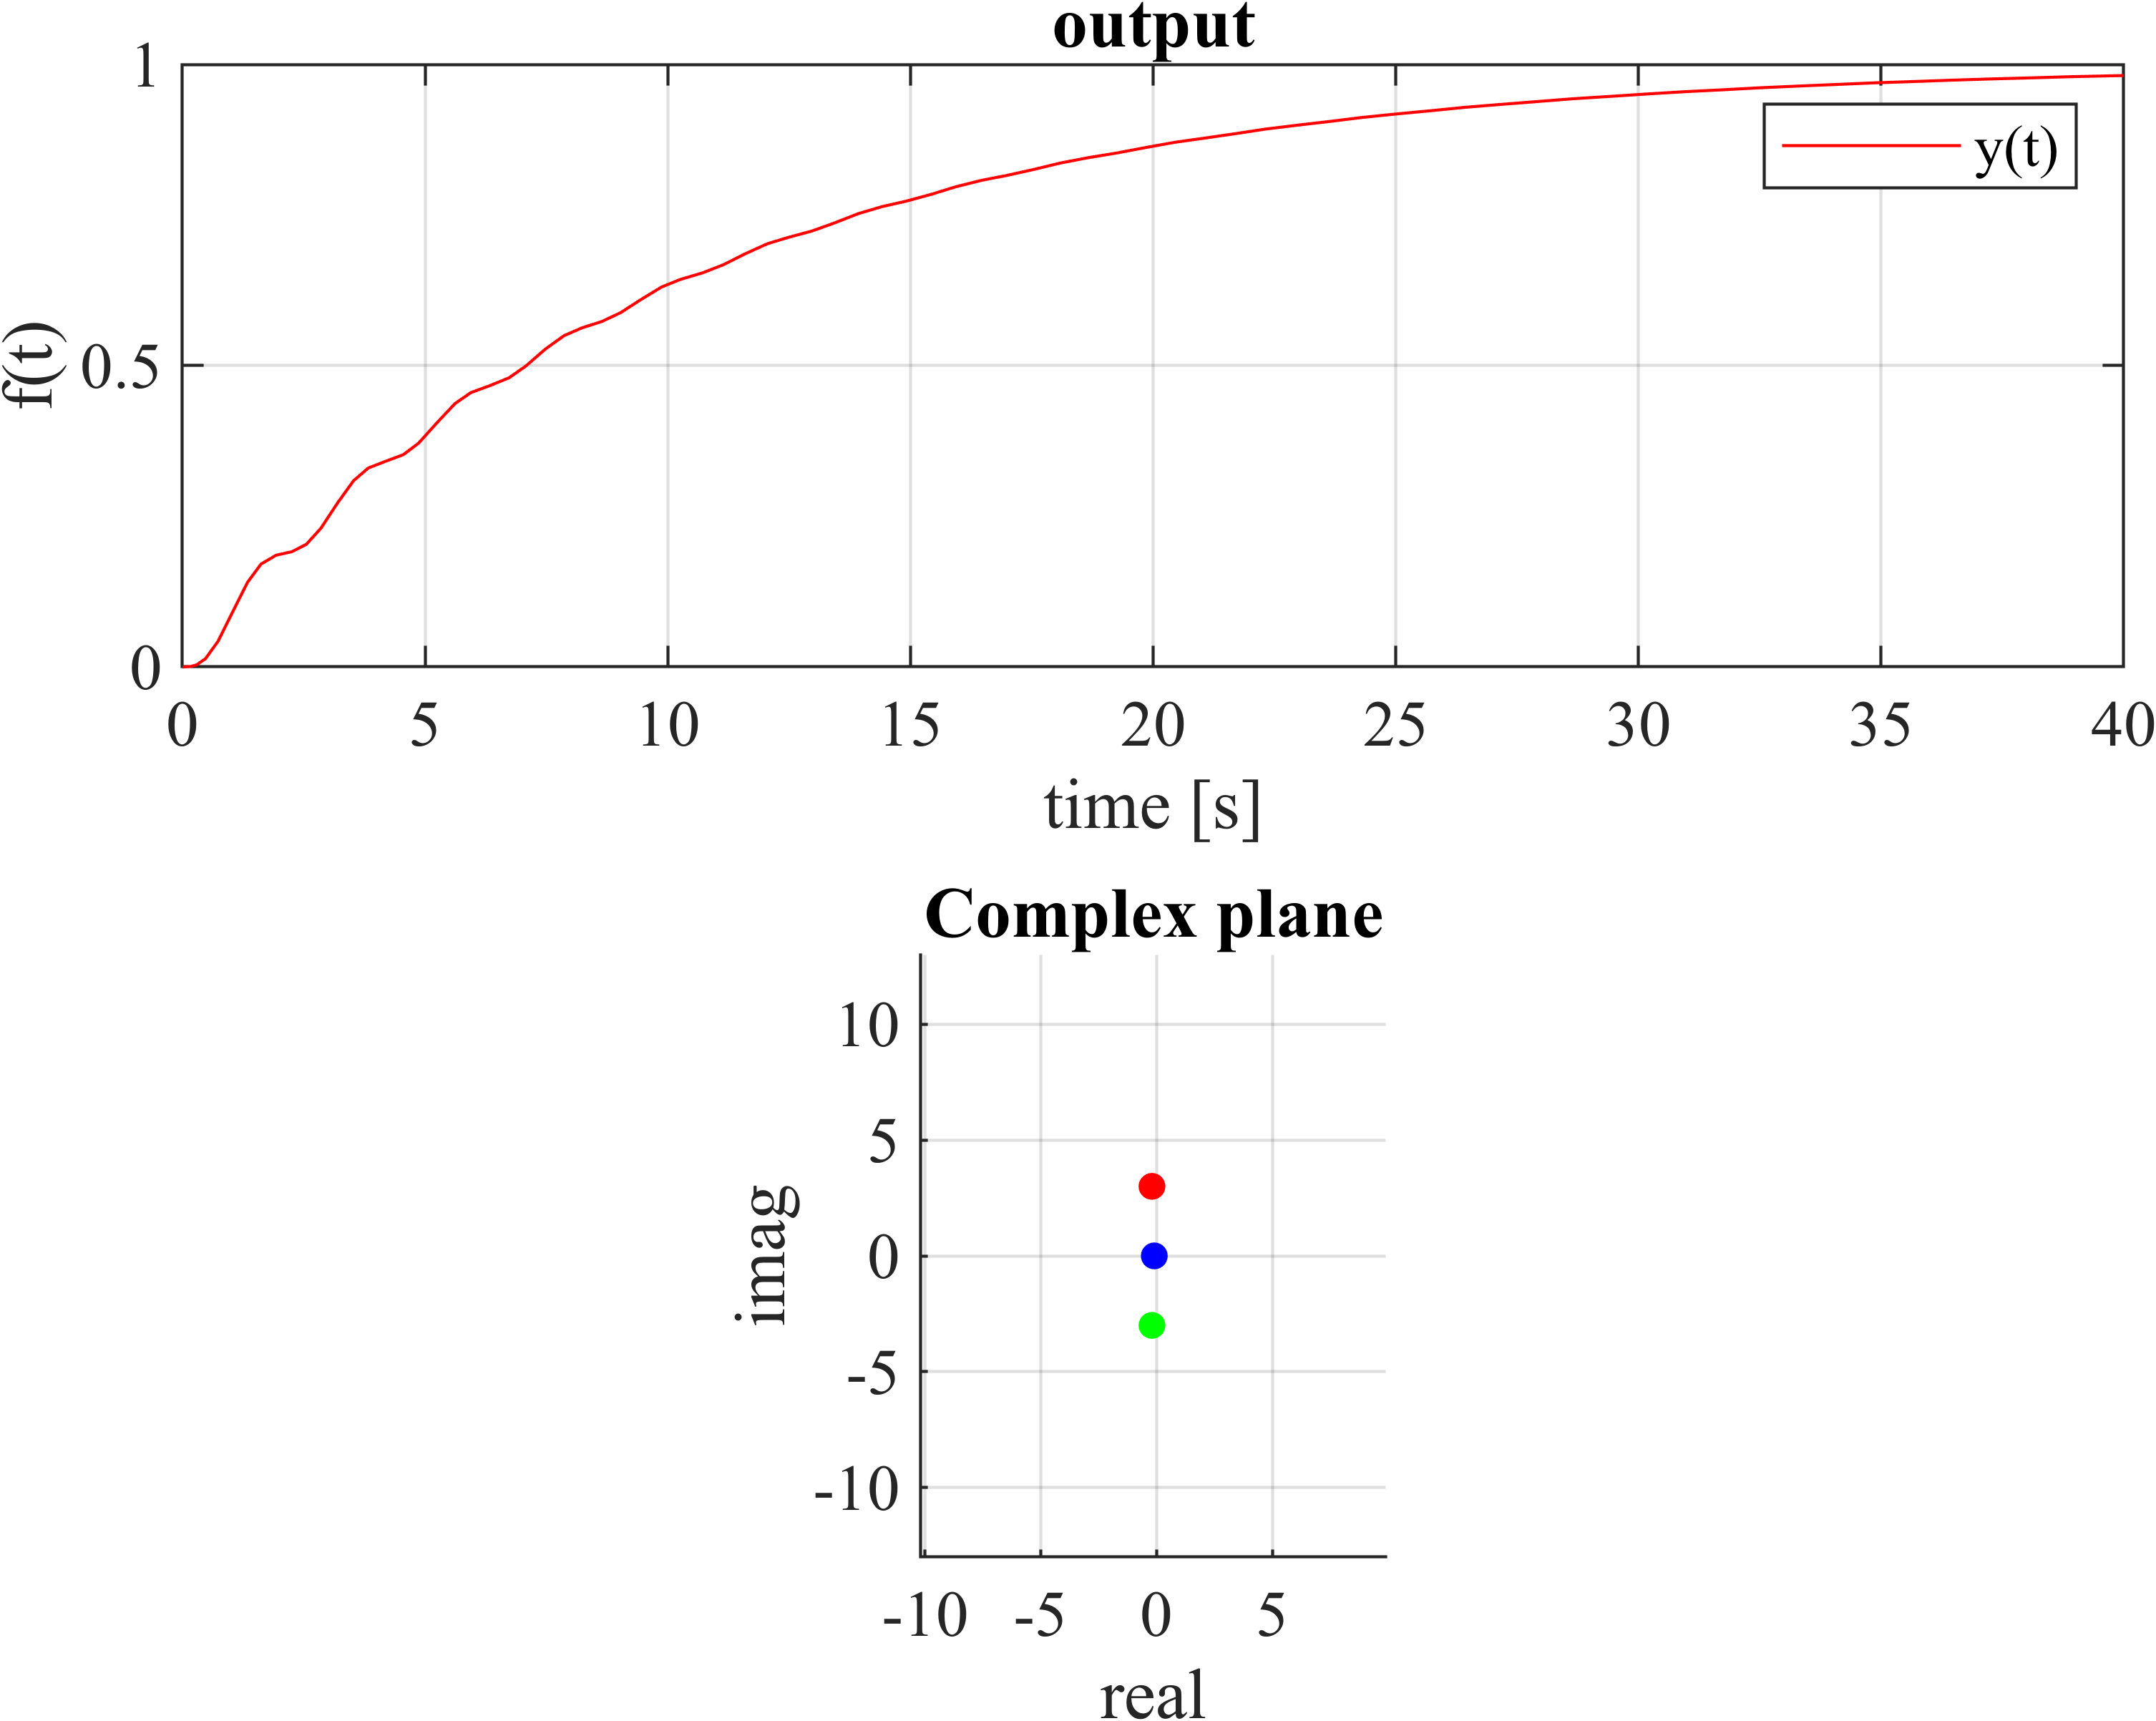
\includegraphics[width=0.8\textwidth]{output_task2_exp11.png}
  \caption{Симуляция - при $\lambda_1 = -0.2 +3i, \lambda_2 = -0.2 - 3i,\lambda_3 = -0.1$}
\end{figure}
Получаем:
$$
\begin{aligned}
  \sigma_{11} \approx 0\% \\
  t_{11} \approx 33.3s
\end{aligned}
$$

\newpage
\section{12-й эксперимент}
\begin{figure}[ht]
    \centering
    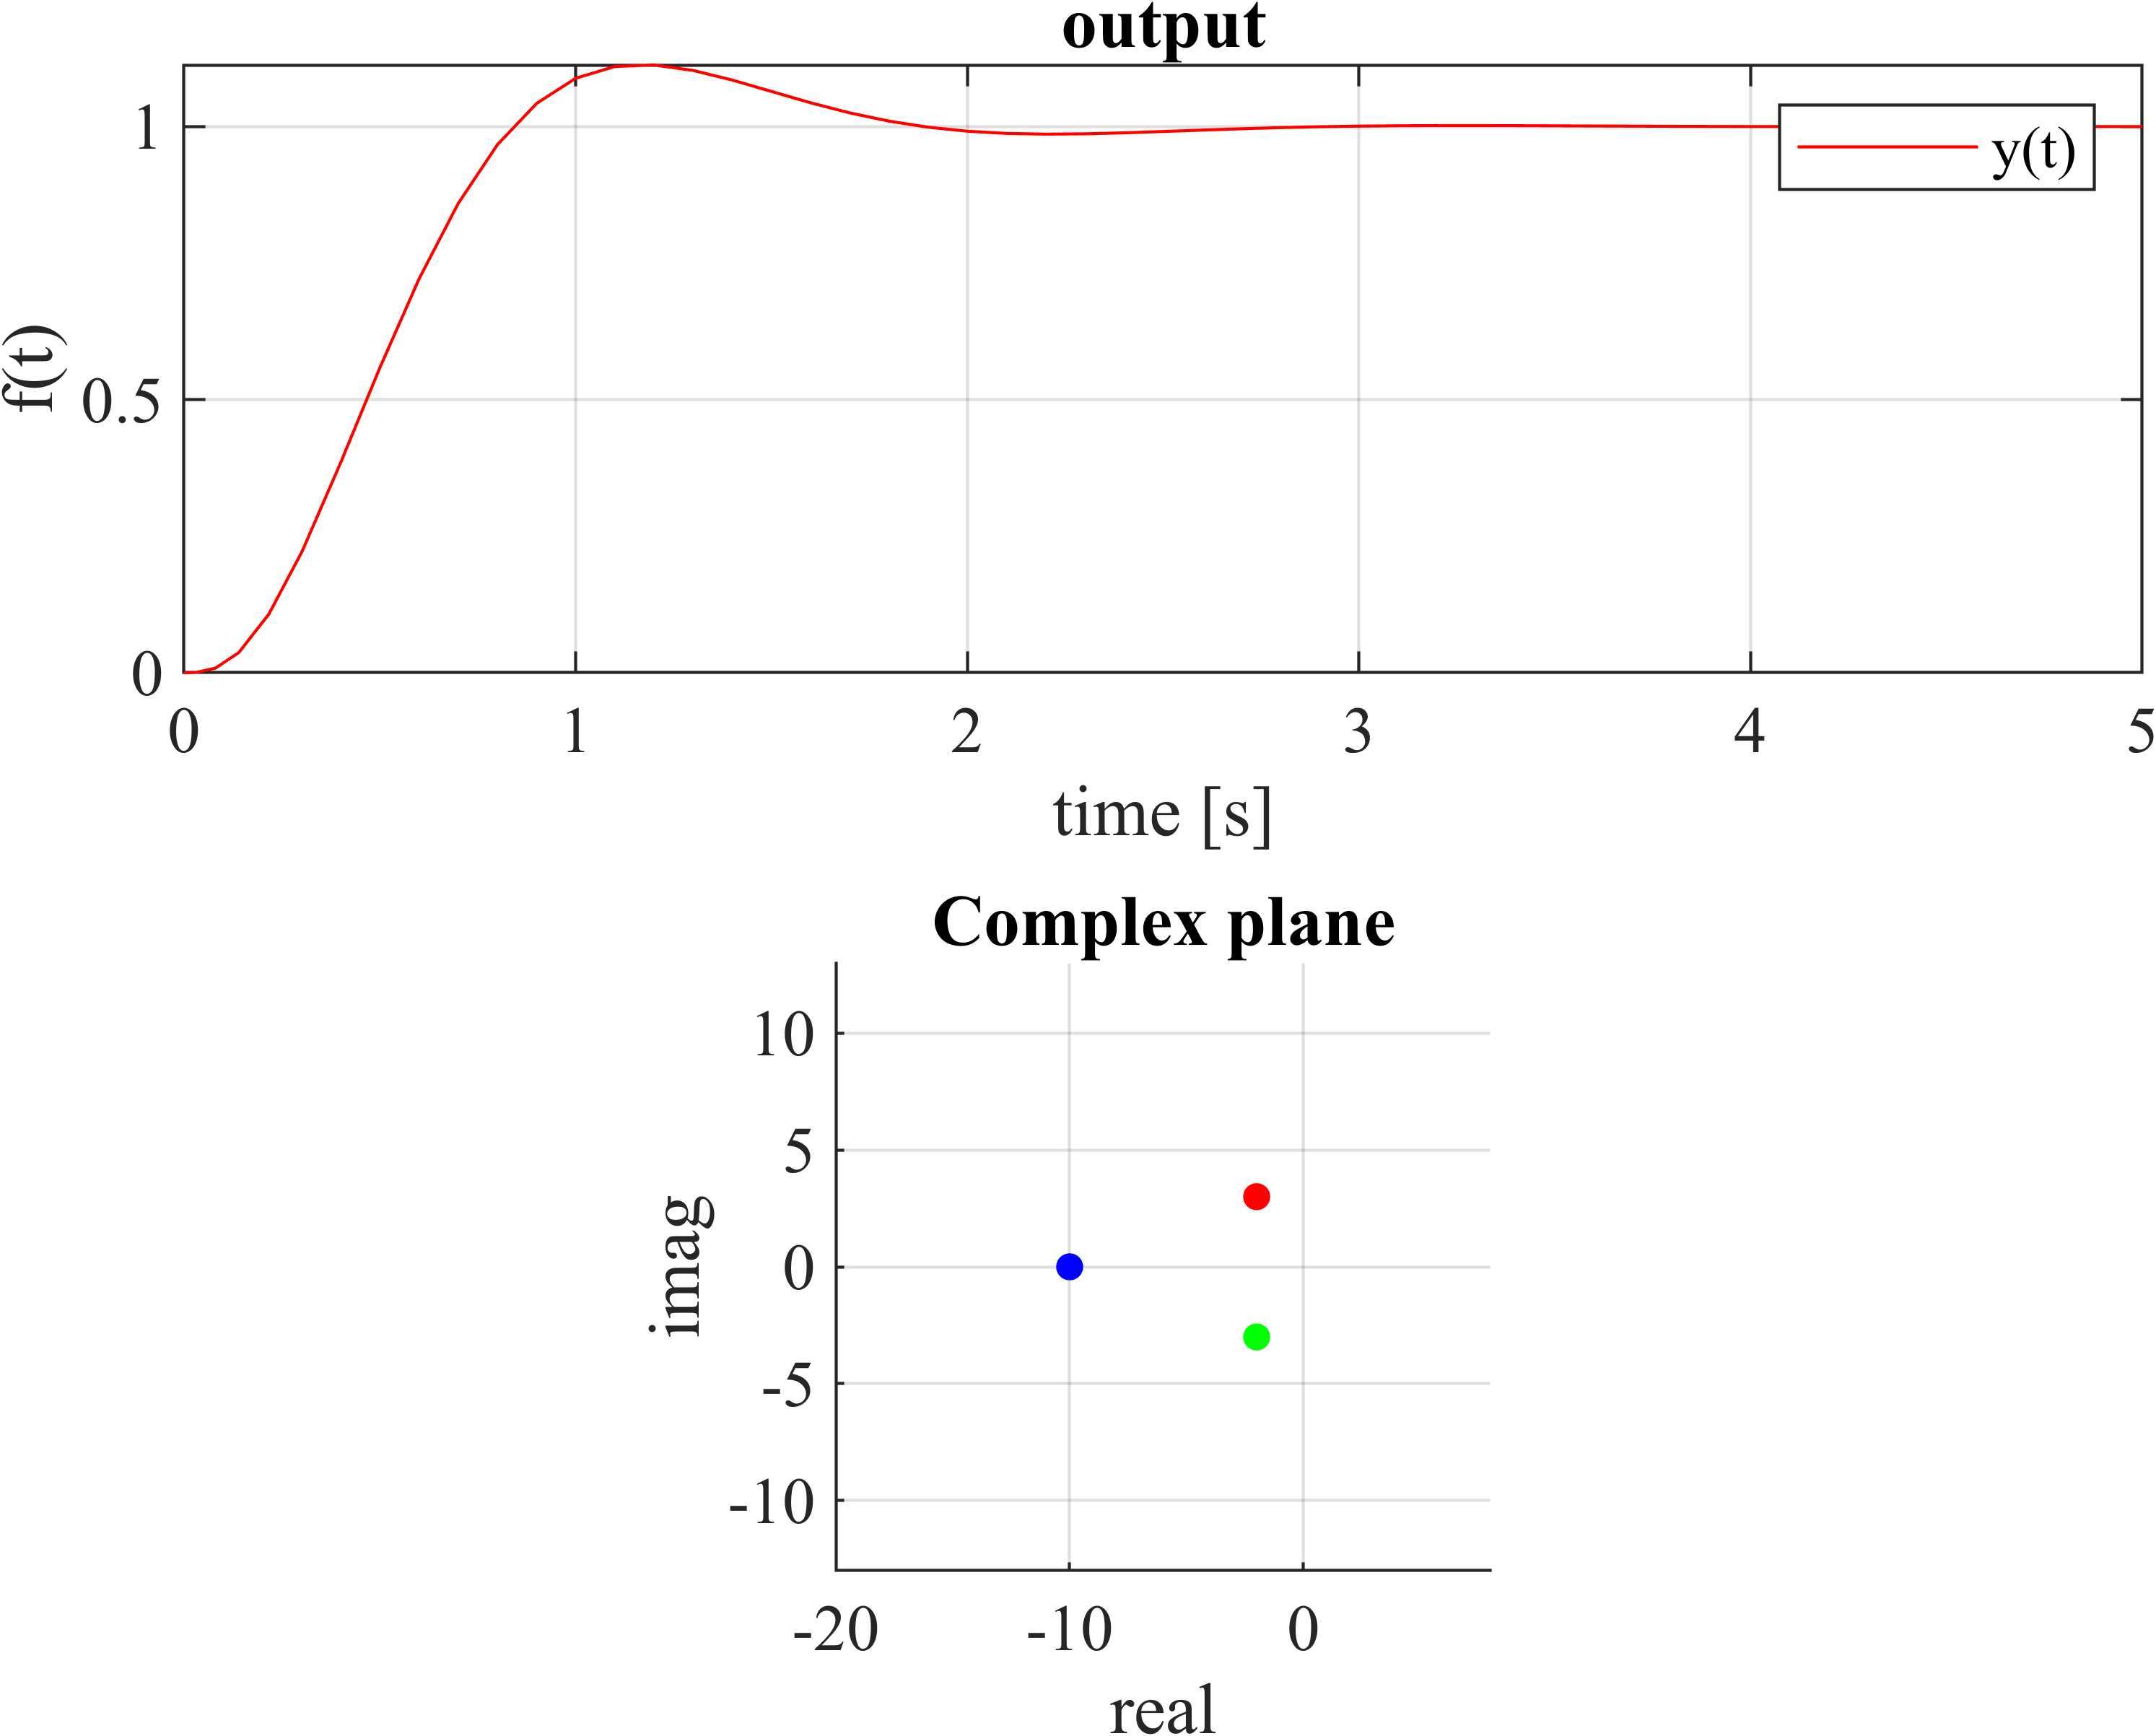
\includegraphics[width=0.8\textwidth]{output_task2_exp12.png}
  \caption{Симуляция - при $\lambda_1 = -2 +3i, \lambda_2 = -2 - 3i,\lambda_3 = -10$}
\end{figure}
Получаем:
$$
\begin{aligned}
  \sigma_{12} \approx 11\% \\
  t_{12} \approx 2.0s
\end{aligned}
$$

\newpage
\section{13-й эксперимент}
\begin{figure}[ht]
    \centering
    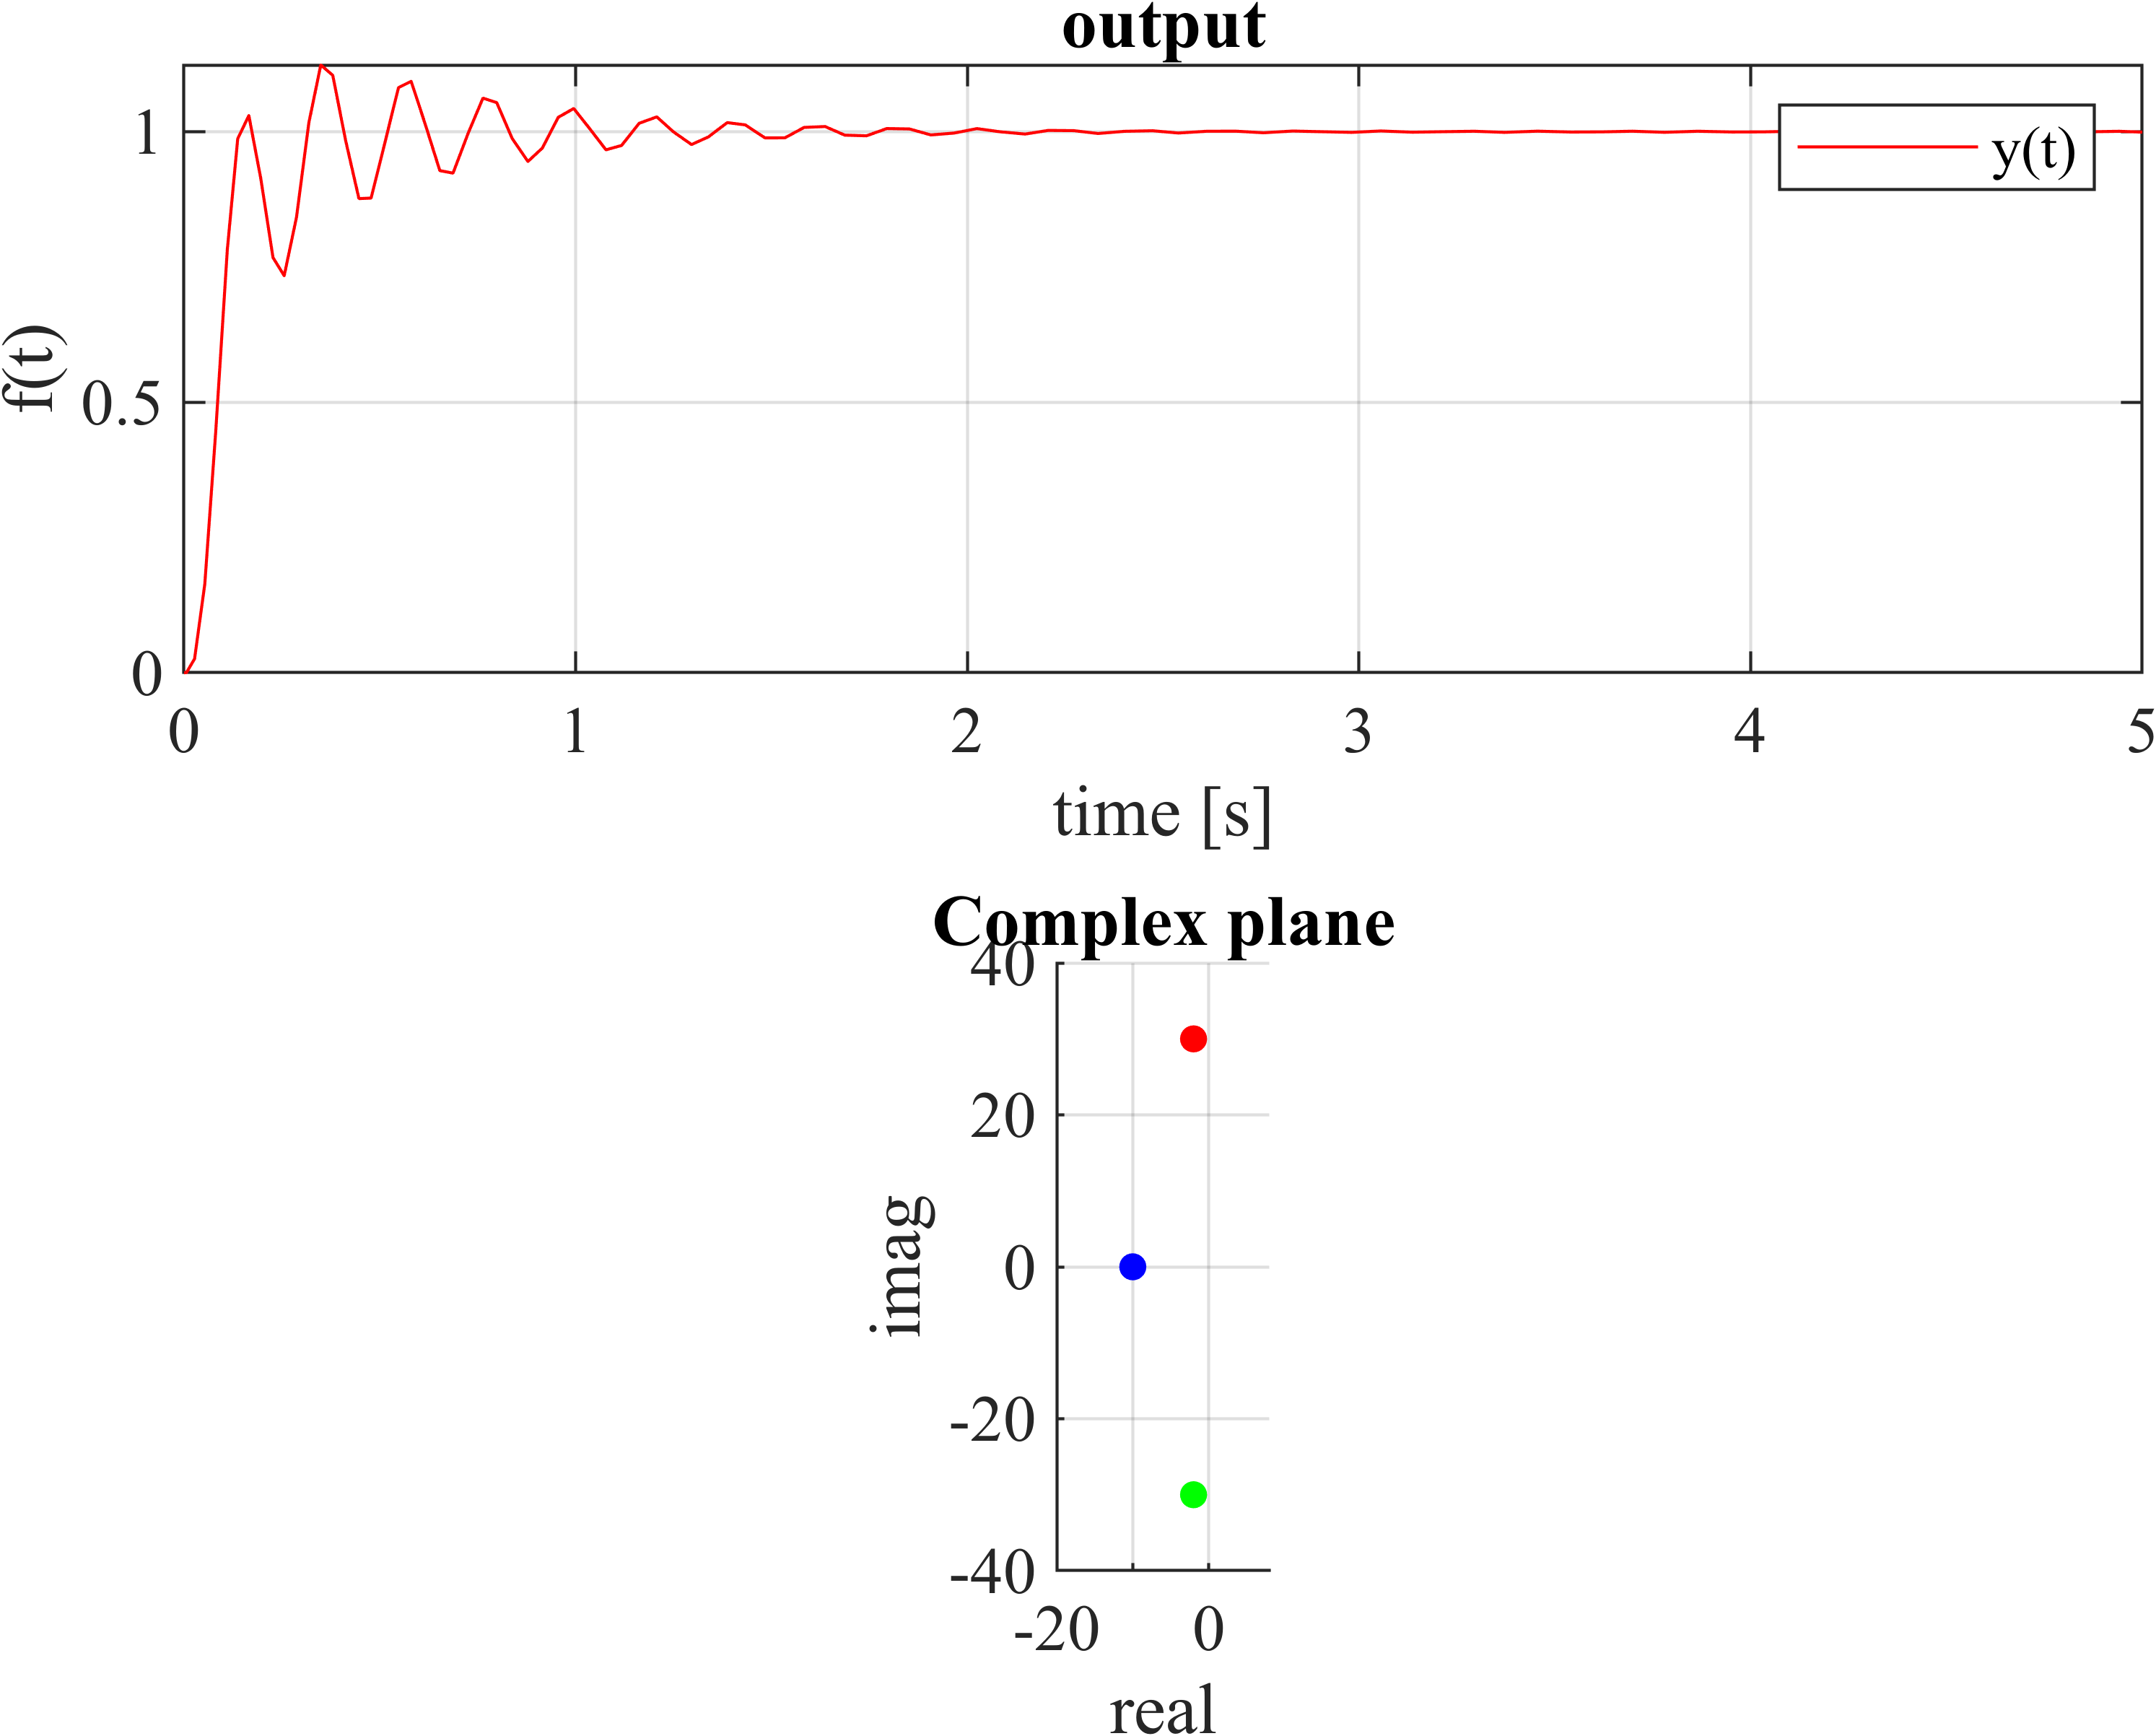
\includegraphics[width=0.8\textwidth]{output_task2_exp13.png}
  \caption{Симуляция - при $\lambda_1 = -2 +30i, \lambda_2 = -2 - 30i,\lambda_3 = -10$}
\end{figure}
Получаем:
$$
\begin{aligned}
  \sigma_{13} \approx 12\% \\
  t_{13} \approx 1.1s
\end{aligned}
$$

\newpage
\section{Выводы}
Сведём полученные результаты в общую таблицу, чтобы упростить себе жизнь:



\begin{table}[h!]
    \centering
    \begin{tabular}{|c|c|c|c|c|c|c|c|c|c|c|}
        \hline
        № & $\lambda_1$ & $\lambda_2$ & $\lambda_3$ & $\sigma,\%$ & $t, \text{s}$ \\
        \hline
        1 & -1 & -2 & -3 & 0 & 5.1 \\
        2 & -1 & -2 & -10 & 0 & 4.8 \\
        3 & -10 & -2 & -3 & 0 & 2.7 \\
        4 & -1 & -20 & -3 & 0 & 4.4\\
        5 & -30 & -20 & -1 & 0 & 4.0\\
        6 & -1 -2i & -1 + 2i & -5 & 18 & 1.2 \\
        7 & -10 & -2 + i & -2 -i & 0.17 & 2.2 \\
        8 & -5 - i & -5 + i & -3 & 0 & 1.8 \\
        9 & -1 -2i & -1 + 2i & -20 & 20 & 1.1 \\
        10 & -20 + 3i & -20 - 3i & -1 & 0 & 4.0\\
        11 & -20 + 3i & -20 - 3i & -1 & 0 & 33.3\\
        12 & -2 + 3i & -2 - 3i & -10  & 11 & 2.0\\
        13 & -2 + 30i & -2 - 30i & -10 & 12 & 1.1\\
        \hline
    \end{tabular}
    \caption{Результат исследования второго задания}
\end{table}

По данным таблицы можно заметить, что перерегулирование появляется только у систем с комплексно-сопряжёнными полюсами. 
Также сделаю предположение, что  при увеличении $|\lambda_1\lambda_2\lambda_3|$ у нас увеличивается перерегулирование, но это работает не для всех случаев. 
Но при уменьшении этого модуля у нас увеличивается время переходного процесса(плохо).

Также по последним двум экспериментам можно заметить, что при увеличении только мнимой компоненты (без злоупотребления) можно заметно уменьшить время переходного процесса, что является подтверждением тезисов с практики 3. Комплексная часть - милое дело.


\endinput